\documentclass[12pt,letterpaper]{article}
\usepackage[utf8]{inputenc}
\usepackage[spanish]{babel}
\usepackage{amsmath}
\usepackage{float}
\usepackage{amsfonts}
\usepackage{amssymb}
\usepackage{graphicx}
\usepackage[left=2cm,right=2cm,top=2cm,bottom=2.5cm]{geometry}
\usepackage{pdfpages}
\usepackage{subfigure}
\author{}
\date{}
\usepackage{fancyhdr}
\pagestyle{fancy}
\fancyhf{}
\fancyhead[RO]{
\includegraphics[width=0.8cm]{figuras/unsl.png}}
\fancyhead[CO]{Universidad Nacional de San Luis\\Facultad de Ciencias Fisico Matemáticas y Naturales}
\fancyfoot[CO]{\emph{Tutorial de manejo de placa EDU CIAA con RTOS OSEK}}
\pagenumbering{arabic}
\fancyfoot[RO]{\thepage}
\begin{document}
%insertar portada
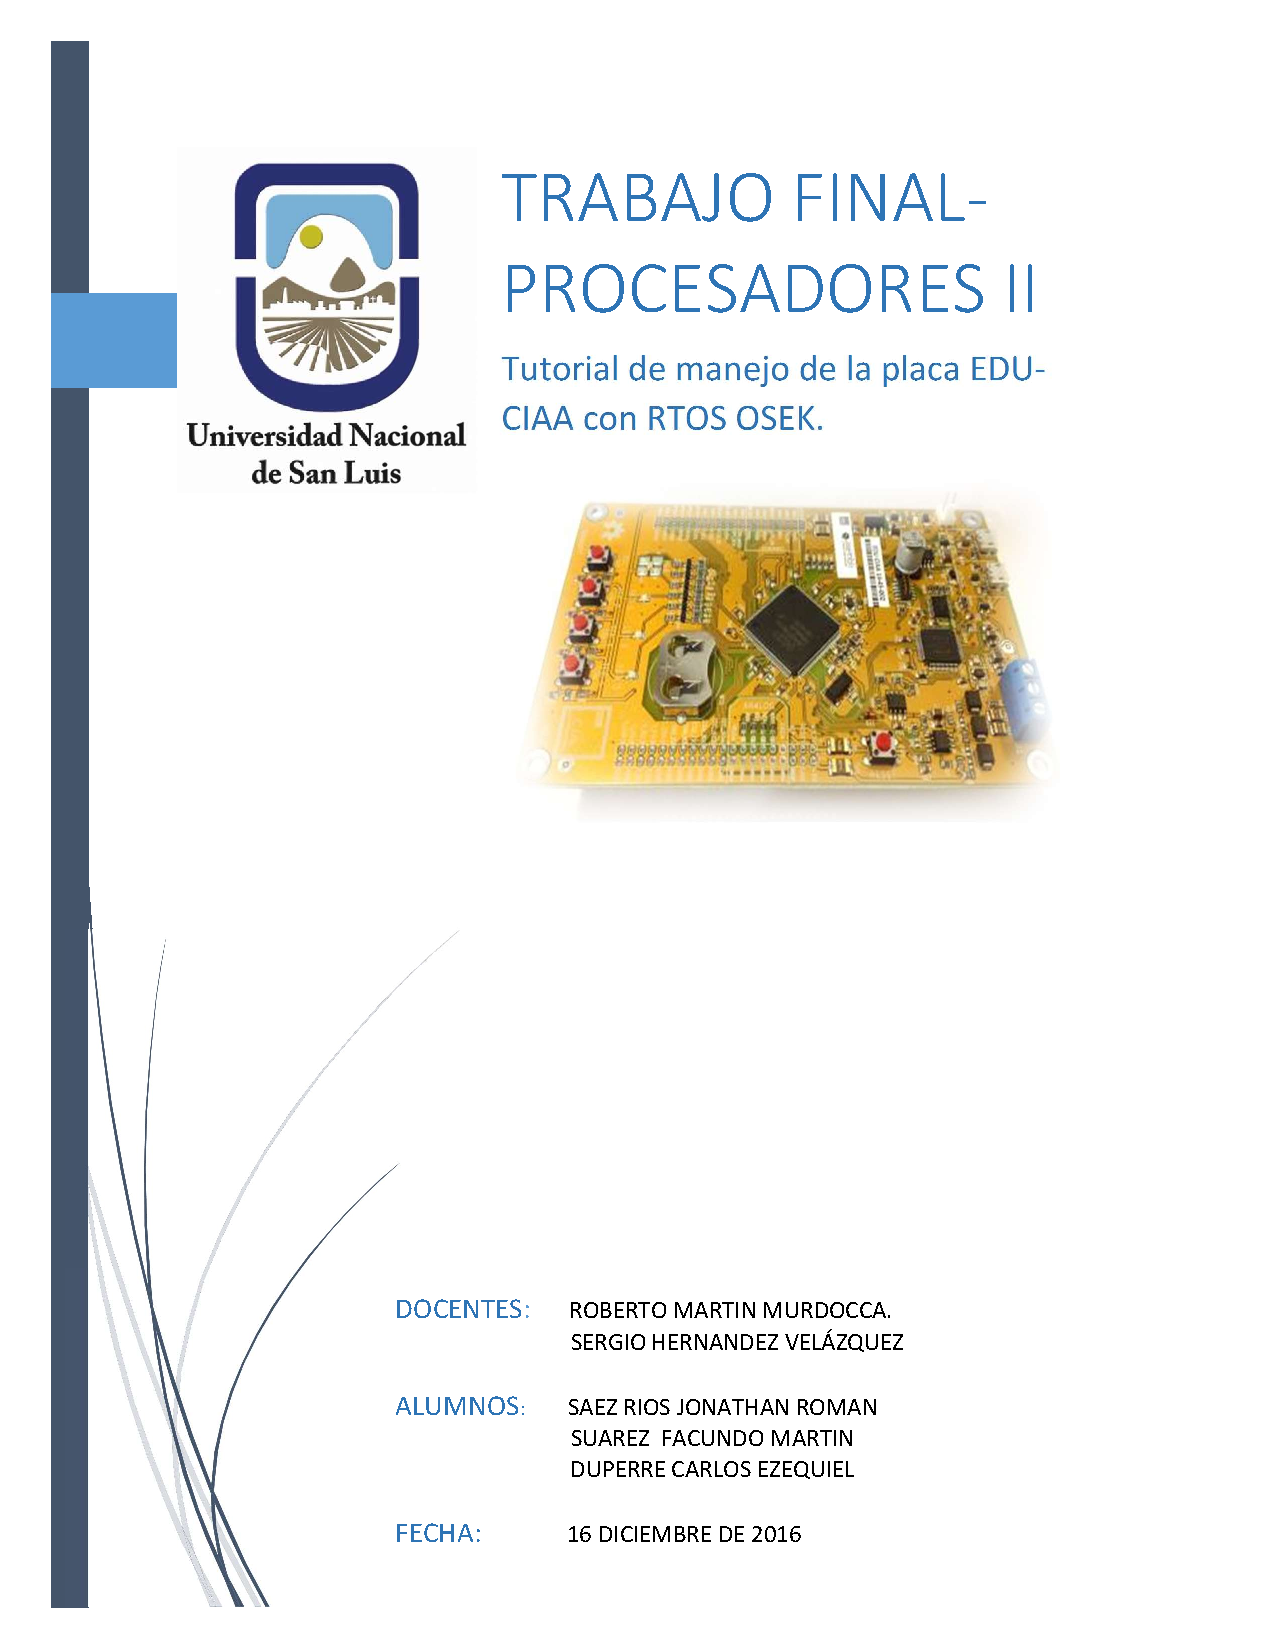
\includepdf{figuras/portada3}

\tableofcontents

\section{Introducci\'on}
En este trabajo se pretende desarrollar un tutorial que permita al usuario poder iniciar sus primeros proyectos usando RTOS y comprender la arquitectura de los microcontroladores Cortex.
  \\
  
Este estudio aborda en primer lugar, las características principales de la placa y la correcta instalación del software sobre Windows 7, Windows 8, y Windows 10 para permitir el desarrollo de códigos sobre ella; además se incluyen posibles problemas que puedan suceder en el proceso junto con sus soluciones.
  \\

La siguiente sección comienza introduciendo al usuario en el uso de la placa a través de la librería \textit{sAPI} (realizada por Eric Pernia) ésta nos permite el desarrollo de programas utilizando lenguaje C. La idea es brindar una explicación simple de la arquitectura de los microcontroladores Cortex y a su vez brindar una base para la siguiente sección del informe.
  \\

Luego, se introduce al usuario en la programación a través de el sistema operativo \textit{OSEK OS}, el cual es el método de programación en el que se proyectó cuando se realizó el diseño de la placa. Se pretende mostrar las bases conceptuales principales de los sistemas operativos en tiempo real, e introducir al usuario a la programación de códigos simples y alentar al usuario a profundizar sobre este estudio.

\subsection{Origen del proyecto CIAA}
Sobre julio de 2013, la Secretaría de Planeamiento Estratégico Industrial del Ministerio de Industria de la Nación (SPEI) y la Secretaría de Políticas Universitarias del Ministerio de Educación de la Nación (SPU) convocaron a la Asociación Civil para la Investigación, Promoción y Desarrollo de los Sistemas Electrónicos Embebidos (ACSE) y a la Cámara de Industrias Electrónicas, Electromecánicas y Luminotécnicas (CADIEEL) a participar en el "Plan Estratégico Industrial 2020". A partir de dicha convocatoria se inició el desarrollo de la Computadora Industrial Abierta Argentina (CIAA).
  \\

El pedido inicial fue que desde el sector académico (ACSE) y desde el sector industrial (CADIEEL) se presenten propuestas para agregar valor en distintas ramas de la economía (maquinaria agrícola, bienes de capital, forestal, textil, alimentos, etc.) a través de la incorporación de sistemas electrónicos en procesos productivos y en productos de fabricación nacional. Debe destacarse que muchas empresas argentinas de diversos sectores productivos no incorporaban electrónica en sus procesos productivos o en sus productos, otras utilizaban sistemas electrónicos obsoletos, muchas utilizaban sistemas importados y sólo unas pocas utilizaban diseños propios basados en tecnologías vigentes y competitivas.
  \\

A partir de esta situación, la ACSE y CADIEEL propusieron desarrollar un sistema electrónico abierto de uso general, donde toda su documentación y el material para su fabricación estuviera libremente disponible en internet, con el objetivo de que dicho sistema pueda ser fabricado por la mayoría de las empresas PyMEs nacionales, y realizar modificaciónes en base a las necesidades específicas que puedan tener.
  \\

Hoy en día la CIAA está disponible en la versión CIAA-NXP y otras seis versiones están en elaboración: CIAA-ATMEL, CIAA-FSL, CIAA-PIC, CIAA-RX, CIAA-ST, CIAA-TI. Además, se está trabajando en el firmware y en el software, para que la CIAA se pueda programar en lenguaje C utilizando una API especialmente diseñada para ser compatible con los estándares POSIX y que sea portable a diversos sistemas operativos de tiempo real.
  \\

Desde la concepción del proyecto, el diseño de la placa se encuentra pensada para soportar las condiciones hostiles de los ambientes industriales los que abundan ruidos, vibraciones, temperaturas extremas, picos de tensión e interferencias electromagnéticas, y además se diseñó de modo tal que pueda ser fabricada en Argentina.

\subsection{Descripción de la placa}

La CIAA es una plaqueta electrónica provista de un microcontrolador y puertos de entrada y salida, cuyo diseño se encuentra disponible en Internet. Esta placa fue concebida para ser utilizada para sistemas de control de procesos productivos, agroindustria, automatización.
 \\
 
La placa EDU CIAA es la versión educativa de la CIAA, la cual se encuentra diseñada con el propósito de conseguir una plataforma base para el desarrollo de proyectos educativos, en este caso, se busca proporcionar las bases del desarrollo de códigos utilizando RTOS. En la Figura \ref{Fig_placa} se puede observar una vista superior de la placa.

\begin{figure}[H]
\centering
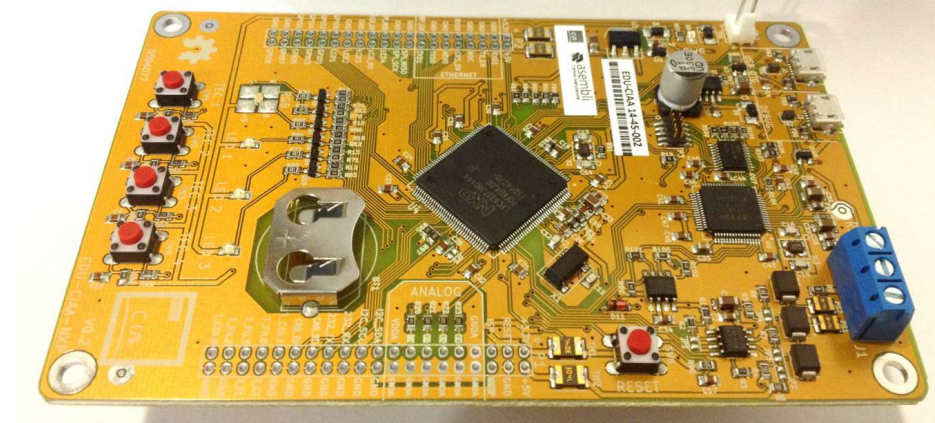
\includegraphics[width=10 cm]{figuras/descripcion1.png}
\caption{Placa EDU CIAA.}
\label{Fig_placa}
\end{figure}

El microcontrolador que utiliza es el LPC4337, que está basado en el ARM Cortex M4. Utiliza una memoria flash de 1MB, memoria de 264 KB de SRAM, memoria ROM de 64 KB, E2PROM de 16 KB, y una memoria OTP de 64 bit.
  \\

La frecuencia de trabajo del procesador alcanza los 204 Mhz. Una característica vital de éste, es que provee soporte para la depuración en JTAG, con posibilidad de incluir hasta 8 breakpoints, y 4 watchpoints.
  \\

El microcontrolador brinda una interface que hace posible extender hasta 164 pines de entrada-salida de propósito general (GPIO), provee una interface USB Host/Device 2.0 de alta velocidad con soporte para acceso directo de memoria, una interface UART 550 con soporte DMA , tres USART 550 con soporte para DMA.
  \\

Como perifericos analógicos, debe destacarse la inclusión de un DAC de 10 bits, con soporte DMA y frecuencia de conversión de 400.000 muestras por segundo. Dos ADC's con soporte DMA, y frecuencia de conversión de 400.000 muestras por segundo, con un numero máximo de 8 canales sobre cada ADC. Y un ADC de 12 bits de 6 canales con soporte DMA, cuya frecuencia de conversión que puede alcanzar hasta los 80 MSamples/s.
  \\

El cristal oscilador posee un rango de operación desde 1 MHz hasta 25 MHz, este microcontrolador incluye un reloj de tiempo real de baja potencia, el cual utiliza un oscilador de cristal.
  \\

La placa provee alimentación de 3,3 V (cuyo rango oscila entre 2,2 V hasta 3,6 V), y es capaz de operar en cuatro modos, los cuales se denominan \textit{sleep}, \textit{deep-sleep}, \textit{power-down},y \textit{deep power-down}. Es posible restablecer la operación de la placa desde los modos \textit{deep-sleep}, \textit{power-down}, y \textit{deep power-down}, a través de interrupciones externas.
 \\
 
La Figura  \ref{Fig2} muestra  una imagen frontal de la placa; nótese la presencia de dos puertos sobre los cuales se ubican los pines correspondientes a la placa.

\begin{figure}[H]
\centering
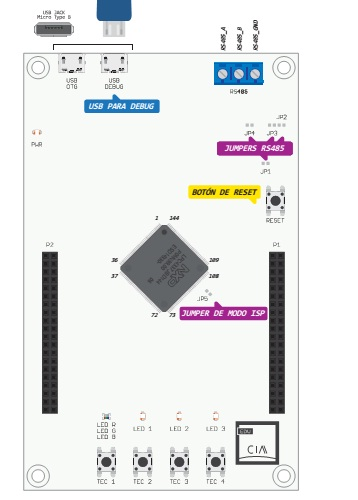
\includegraphics[width=6 cm]{figuras/FIGURA_1.jpg}
\caption{Imagen frontal de placa.}
\label{Fig2}
\end{figure}
 
En la Figura  \ref{diagramaenbloques} puede observarse el diagrama en bloques de la placa, puede notarse que la placa cuenta con 2 puertos micro-USB (uno para aplicaciones y debugging, otro para alimentación); 4 salidas digitales implementadas con leds RGB, 4 entradas digitales con pulsadores; 1 puerto de comunicaciones RS485 con bornera. 
\begin{figure}[H]
\centering
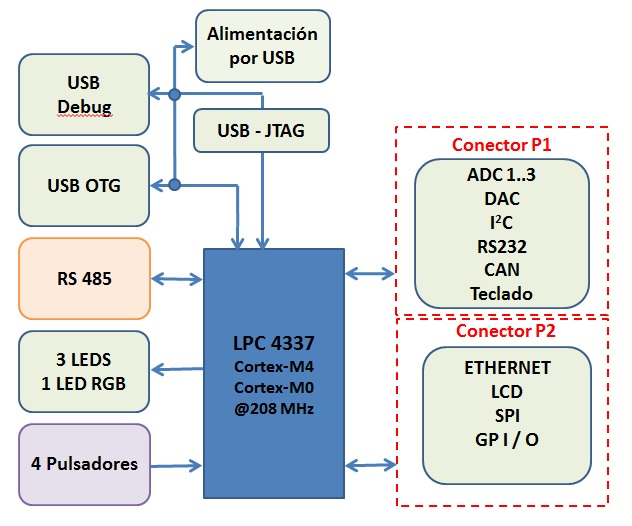
\includegraphics[width=8 cm]{figuras/diagramaenbloques.jpg}
\caption{Diagrama en bloques de EDU CIAA basado en LPC4337.}
\label{diagramaenbloques}
\end{figure}
La Figura  \ref{distribucionpines} ilustra el distribución de los pines sobre cada puerto.
\begin{figure}[H]
\centering
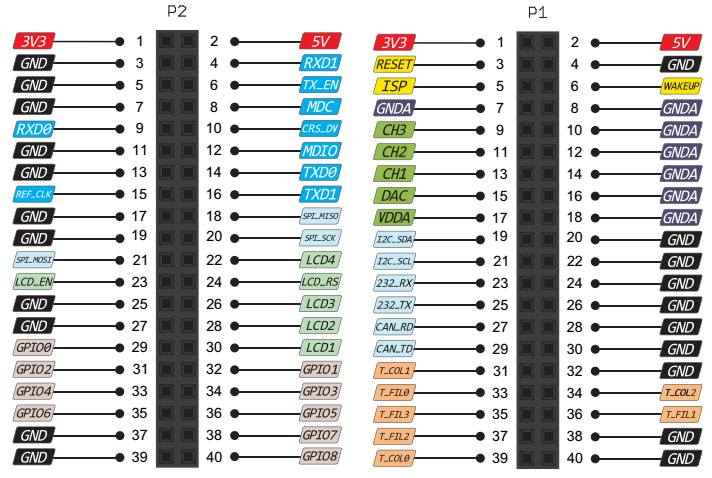
\includegraphics[width=8 cm]{figuras/f16.png}
\caption{Distribución de pines de la placa.}
\label{distribucionpines}
\end{figure} 
Sobre el puerto P1, se ubican los siguientes módulos:

\begin{enumerate}
\item[•] 3 entradas analógicas (ADC0,1,2 y 3)
\item[•] 1 salida analógica (DAC0).
\item[•] 1 puerto I2C.
\item[•] 1 puerto asincrónico full duplex (para RS-232).
\item[•] 1 puerto CAN.
\item[•] 1 conexión para un teclado 3x4.
\end{enumerate}

Sobre el puerto P2, se ubican los siguientes módulos:

\begin{enumerate}
\item[•] 1 puerto Ethernet
\item[•] 1 puerto SPI
\item[•] 1 puerto para Display LCD con 4 bits de datos, Enable y RS.
\item[•] 8 pines genéricos de I/0.
\end{enumerate}

\section{Instalacion de Software}

\subsection{Conceptos previos}
El desarrollo de codigos para sistemas embebidos tiene ciertas semejanzas con el desarrollo de aplicaciones en las PC, en este caso particular se utiliza un compilador llamado \textit{GCC} con soporte para la compilación de proyectos sobre los microcontroladores basados en la arquitectura ARM. En este caso particular, el compilador utilizado para la EDU CIAA se lo denomina \textit{arm-none-eabi-gcc}.
 \\
 
Para la ejecución de la depuración de algún programa previamente compilado, el hardware de la CIAA viene provisto con el chip \textit{FT2232H}, que se encarga de hacer un puente entre la interfase JTAG del microcontrolador, y el USB que conecta a la PC en el puerto USB dedicado al debug. Mediante la herramienta de código abierto \textit{OpenOCD (On Chip Debugger)} se controla el chip \textit{FT2232H} por el USB y ademas todo lo referido al JTAG. Luego la herramienta de depuración \textit{GDB} utilizado en el IDE-Eclipse (Entorno de Desarrollo Integrado) que se instala, se comunica sobre el puerto 3333 (TCP) que el \textit{Open OCD} tiene en escucha esperando la conexión.
 \\
 
Debe tenerse en cuenta que el chip \textit{FT2232H} posee 2 canales de comunicación independientes (A y B), sin embargo, ambos salen por el mismo USB, de modo que la PC detecta 2 dispositivos distintos (en realidad es uno compuesto). Uno de ellos, se conecta al JTAG manejado por \textit{OpenOCD} como fue mencionado, mientras que el otro se ve como un puerto virtual COM. Este último sirve principalmente para la depuración.
 \\

Dado que al funcionar como dos dispositivos distintos, para cada uno de ellos debe realizarse la instalación de un driver adecuado, en principio debe optarse por realizar la instalación de los drivers por defecto del fabricante FTDI para puerto virtual. %Considerar%

\subsection{Firmware de la EDU CIAA}
 
A diferencia de otras placas, como por ejemplo, la \textit{MCE Debug}, en donde se tiene un entorno de trabajo previamente optimizado, en este caso, el software IDE de la EDU CIAA trabaja de forma ligeramente distinta. El usuario debe modificar un archivo \textit{makefile} (basándose en un archivo proporcionado previamente, denominado \textit{Makefile.config}) para poder efectuar la compilación del archivo y lograr la correcta configuración del programa, sobre la placa EDU CIAA. Dentro de él se establece la configuración para la arquitectura del microcontrolador utilizado.
 \\
 
Cuando se desea realizar el primer proyecto sobre la placa, el usuario debe crear su propio archivo \textit{Makefile.mine}, de manera que éste se encuentra basada en \textit{Makefile.config} brindado previamente al momento de establecer un nuevo proyecto añadiendo un Firmware que ha sido diseñado para el funcionamiento de la placa.
 \\
 
Debe tenerse en cuenta que la dinámica de trabajo sobre la placa se encuentra pensada para trabajar sobre la plataforma de versionado \textit{Git}; en este caso en particular, el archivo \textit{Makefile.mine} se encuentra diseñado de forma tal que dicho archivo sea ignorado al sincronizar su repositorio local, con su repositorio remoto (ubicado sobre \textit{Github}).
 \\
 
En \textit{Makefile.mine} se pueden editar y configurar los siguientes parámetros:
\begin{enumerate}
\item[•] \textbf{ARCH}  indica la arquitectura del hardware para la cual se desea compilar. Ej: x86, cortexM4.
\item[•] \textbf{CPUTYPE} indica el tipo de CPU. Ej: none, ia32, ia64, lpc43xx.
\item[•] \textbf{CPU} indica la CPU para la que se desea compilar. Ej: none, lpc4337.
\item[•] \textbf{COMPILER }es el compilador a utilizar. Ej: gcc.
\item[•] \textbf{BOARD }es la placa sobre la cual se trabajaca (CIAA-NXP, EDU-CIAA-NXP, etc.)
\item \textbf{PROJECT }es el Path al proyecto a compilar. Ej: examples$\$(DS)blinking_base$.
\end{enumerate}
Se utiliza la variable \$(DS) para indicar el separador de directorios (de manera automática se usa ``/'' para linux y ``\textbackslash{}'' para Windows 7, 8 y 10).
 \\
 
En el mismo Makefile aparecen al comienzo comentarios donde se indican los valores que pueden tomar estos parámetros.
 \\
 
Otro concepto importante que se tiene en cuenta cuando se desarrollan proyectos propios, es que cada proyecto tiene también su propio archivo \textit{Makefile}.El mismo se encuentra bajo el directorio \textbf{mak} en el directorio principal del proyecto o ejemplo. En el ejemplo \textbf{examples/blinking} el makefile del ejemplo se encuentra en \textbf{examples/blinking/mak} y se llama \textbf{Makefile}.
 \\
 
Sobre este archivo \textit{Makefile} contiene las siguientes definiciones:

\begin{enumerate}
\item[•] \textbf{PROJECT} el nombre del proyecto y por ende nombre del ejecutable.
\item[•] \textbf{\$(PROJECT)$\_$PATH} es el directorio del proyecto.
\item[•] \textbf{INCLUDE} los paths a indicar al compilador para buscar includes files.
\item[•] \textbf{SRC$\_$FILES} archivos a compilar ya sean archivos c como c++.
\item[•] \textbf{OIL$\_$FILES} configuración del sistema operativo (si es utilizado).
\end{enumerate}
Cada proyecto incluye en su Makefile los módulos a compilar en una variable llamada MODS, por ejemplo:\textit{posix}, \textit{ciaak}, \textit{config}, \textit{bsp}, y \textit{platforms}.
 \\

Es recomendable utilizar ``\$(DS)'' en vez de ``/'' o ``\textbackslash{}'' para mantener la compatibilidad entre sistemas operativos (Linux, Windows, MAC OS).
{
\subsection{Estructura de Directorios de Firmware de EDU CIAA}
La Figura \ref{Fig3} ilustra los contenidos de la estructura de directorios.
\begin{figure}[H]
\centering
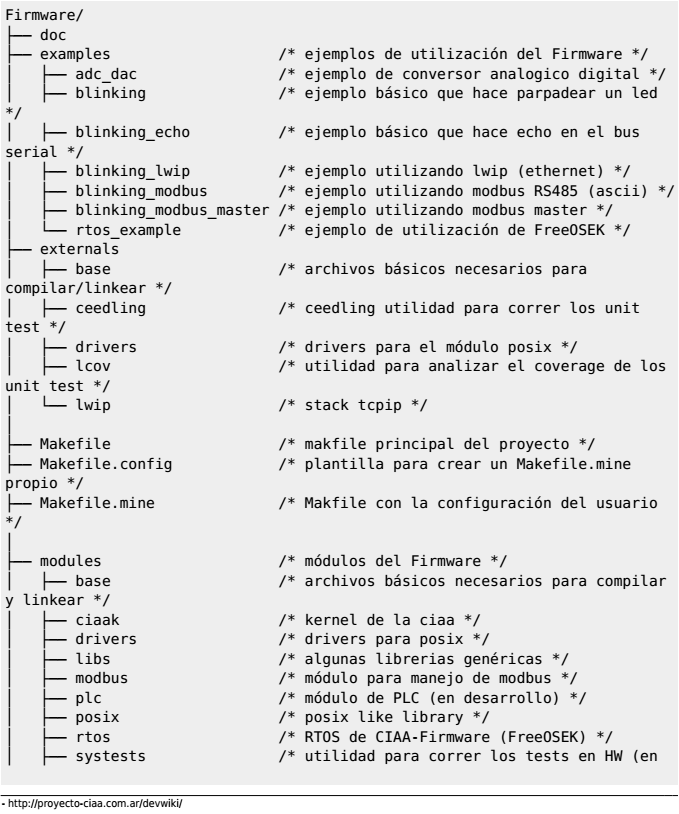
\includegraphics[width=10 cm]{figuras/est_directorios_ciaa.png}\\
\caption{Estructura de directorios del Firmware.}
\label{Fig3}
\end{figure}

En el directorio principal luego de hacer un git clone o al bajar una release oficial se pueden encontrar los siguientes Directorios y Archivos:

\textbf{Directorio $"externals"$(Software y Tools Externos)}::
 \\
 
Este directorio contiene el Software y Tools externos al CIAA-Firmware, que son necesarios para compilar, testear, etc. el Firmware. Tenga en cuenta que el Software y Tools en esta carpeta no son parte de CIAA-Firmware y pueden contener otras licencias. Sobre el Cuadro \ref{Tab1} se ilustra los contenidos del directorio y su descripción, mientras que el Cuadro \ref{Tab2} contiene todos los archivos generados por el CIAA-Firmware.
\begin{table}[H]

\resizebox{16cm}{!}{
\begin{tabular}{|l|l|}
\hline\hline
ceedling & Tool utilizada para los Unit Tests o Pruebas Unitarias\\ \hline
base & Fuentes, headers y linker scripts necesarios para poder compilar y linkear el código en la plataforma\\ \hline
drivers & Drivers provistos por el proveedor del chip, los cuales son luego adaptados al formato de la CIAA.\\ \hline
\end{tabular}
}
\caption{Utilidades,archivos,y drivers para la placa.}
\label{Tab1}

\end{table}
\begin{table}[H]

\resizebox{16cm}{!}{
\begin{tabular}{|l|l|}
\hline\hline
bin & Contiene el binario del proyecto, es el archivo que se va a correr en la PC o a cargar en el CIAA-Firmware\\ \hline
gen & Archivos generados de OSEK RTOS\\ \hline
lib & Por cada Módulo el make genera un archivo .a, osea una libreria\\ \hline
obj & Todos los archivos fuentes son compilados a object files y almacenados en este directorio\\ \hline
\end{tabular}
}
\caption{Descripción de archivos generados en un proyecto en RTOS.}
\label{Tab2}

\end{table}
}

\subsection{Iniciación a través de ejemplos}
El Firmware es el conjunto de instrucciones que se ejecuta en la CPU del microcontrolador que comprende los módulos de código de programas para realizar una aplicación determinada, e interactúa directamente con los periféricos internos y otros componentes físicos del microcontrolador.
  \\
  
En el Firmware de la placa se pueden encontrar varios ejemplos, estos se encuentran en la carpeta \textbf{examples} y pueden ser utilizados como base para iniciar cualquier proyecto.
 \\
 
Cualquiera de los ejemplos puede ser copiado y utilizado de base para nuevos proyectos. Por ejemplo con el siguiente comando:	\textit{cp -r $examples/blinking projects/my$\_$proyect$} y adaptando el Makefile.mine indicado, por ejemplo a la dirección: $PROJECT$\_$PATH = projects/my$\_$project$.
\subsection{Instalación de IDE}
El IDE posibilita el trabajo en un ambiente ameno, además provee las herramientas necesarias para el desarrollo de aplicaciones en el Firmware de forma automatica. La CIAA utiliza una versión modificada de la plataforma de software (IDE)  \textit{Eclipse}, denominada \textit{CIAA-Software-IDE} , la cual contiene herramientas de programación tales como editor de texto, compilador, plataforma para depuración, etc.
Sobre la página web del proyecto (\textit{http://proyecto-ciaa.com.ar/}), se provee un instalador llamado \textit{CIAA-IDE-SUITE}, desde donde se puede configurar automáticamente todas las herramientas necesarias para trabajar con la placa. Este instalador solamente es para los usuarios que poseen Windows XP o superior.
 \\

El paquete de instalación incluye:
\begin{enumerate}
\item[•] \textbf{Eclipse}
\item[•]\textbf{PHP (Hypertext Pre-processor )} es un lenguaje de programación de uso general de código desde el lado del servidor, originalmente diseñado para el desarrollo de contenido dinámico. En este caso, se utiliza solamente en forma de scripts para poder generar algunos archivos del \textbf{Sistema Operativo OSEK}
\item[•] \textbf{Cygwin} es una consola que se ejecuta en Windows, de modo de emular la consola de comandos de Linux. Cuenta con todos los comandos, y el compilador GCC, propio del sistema operativo libre.
\end{enumerate}
Para realizar la instalación del IDE, es necesario realizar los siguientes pasos:
\begin{enumerate}
\item[•]\textbf{Paso 1}: Una vez realizada la descarga del instalador, se ejecuta dicha aplicación, la Figura \ref{Fig4} muestra el arranque del instalador, sobre ella, debe seleccionarse \textit{Siguiente}.
\begin{figure}[H]
\centering
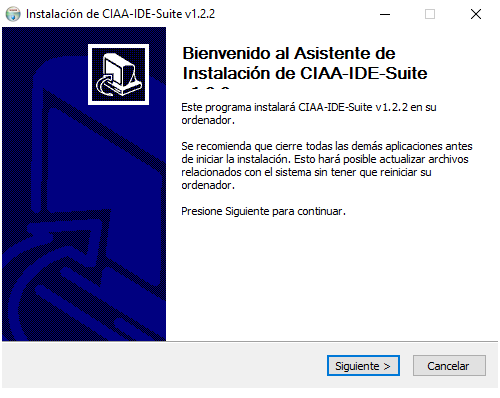
\includegraphics[width=8 cm]{figuras/instalacion1.png}\\
\caption{Arranque del instalador del software IDE}
\label{Fig4}
\end{figure}
\item[•]\textbf{Paso 2}: A continuación, el usuario debe aceptar las licencias para la utilización del programa. Como se muestra en La Figura \ref{Fig5}.
\begin{figure}[H]
\centering
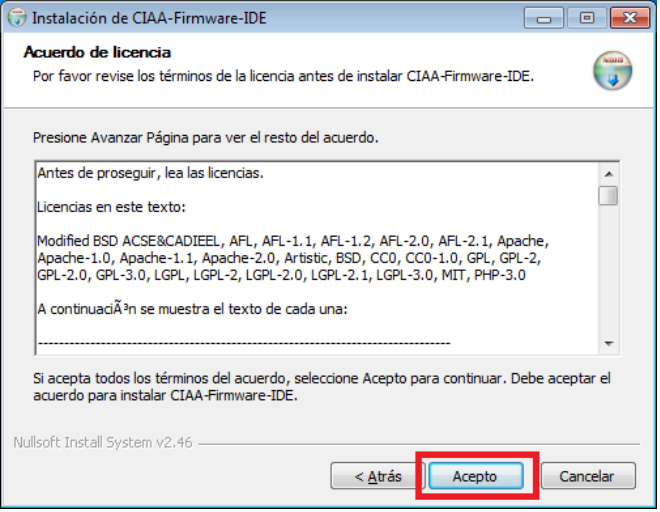
\includegraphics[width=8 cm]{figuras/instalacion2.png}\\
\caption{Arranque del instalador del software IDE.}
\label{Fig5}
\end{figure}
\item[•]\textbf{Paso 3}: Luego se presenta una ventana como la de la Figura \ref{Fig6}, sobre ella deben elegirse cuáles componentes se desean instalar. En el caso que el usuario no cuente con la placa, no es necesario instalar los drivers. En el momento de contar con ella, los drivers se instalan junto con el IDE, los mismos quedarán en la carpeta de destino para su instalación en forma manual; otra forma de instalar los  los controladores es ejecutar el instalador del CIAA-IDE Suite y tildar únicamente la opción \textbf{drivers} al momento de seleccionar los componentes a instalar. 
\begin{figure}[H]
\centering
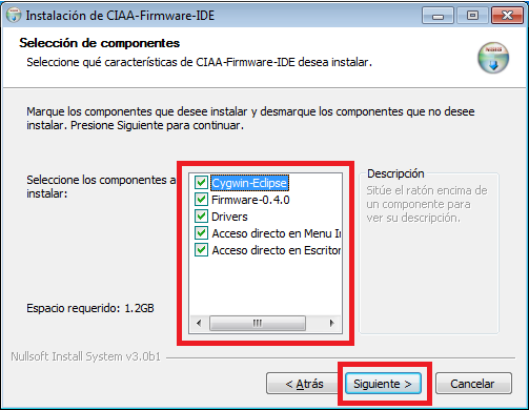
\includegraphics[width=8 cm]{figuras/instalacion3.png}\\
\caption{Selección de componentes del instalador.}
\label{Fig6}
\end{figure}
\item[•]\textbf{Paso 4}: A continuación debe  establecerse la dirección en donde se desea instalar el entorno. La ventana que corresponde a este proceso se ilustra en la Figura \ref{Fig7}. En caso de que se desee cambiar dicha dirección, debe tenerse la precaución de no elegir una dirección donde los directorios posean espacios en sus nombres. Es recomendable no cambiar la unidad de instalación, pues en los siguientes pasos del documento se utilizarán direcciones que harán referencia a esta carpeta de instalación, y si se modifica, se deberán cambiar consecuentemente dichas direcciones.
\begin{figure}[!h]
\centering
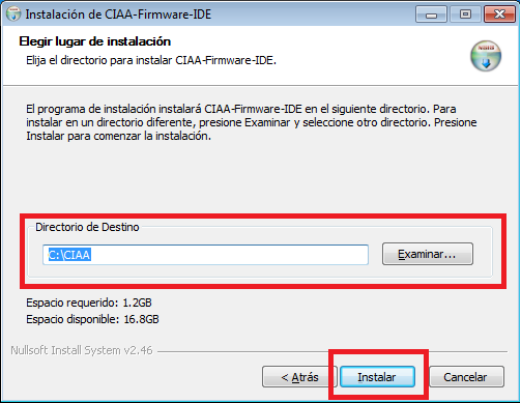
\includegraphics[width=8 cm]{figuras/instalacion4.png}\\
\caption{Elección de la ruta de instalación.}
\label{Fig7}
\end{figure}

\item[•]\textbf{Paso 5}: Luego de dicha configuración, se inicia automáticamente el proceso de instalación. En un momento aparecerá una ventana emergente, similar a la que se muestra en la Figura \ref{Fig8}, en donde el programa pregunta si se dispone del hardware, pues para la instalación del driver es necesario conectar la placa.
\begin{figure}[!h]
\centering
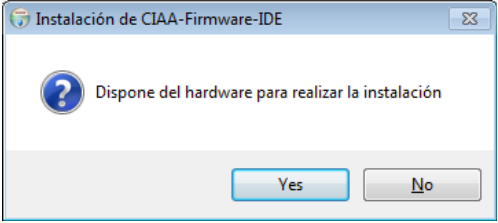
\includegraphics[width=6 cm]{figuras/instalacion5.png}\\
\caption{Instalación de los drivers: primera instancia.}
\label{Fig8}
\end{figure}
\begin{enumerate}
\item[•]\textbf{Paso 5.1}: Si se dispone de la EDU-CIAA, se debe hacer click en 'Yes', y emergerá otra ventana, como se muestra en la Figura \ref{Fig9}.
\begin{figure}[!h]
\centering
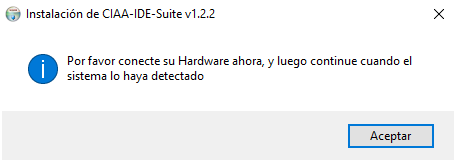
\includegraphics[width=6 cm]{figuras/instalacion6.png}\\
\caption{Instalación de drivers si se dispone del hardware.}
\label{Fig9}
\end{figure}
\item[•]\textbf{Paso 5.2}: Una vez finalizada esta etapa, se procede a la instalación de los drivers por defecto del fabricante FTDI para puerto virtual. Este proceso se ilustra en las figuras \ref{driversFTDI} , \ref{Fig10}, \ref{Fig11} y \ref{Fig12}.
\begin{figure}[H]
\centering
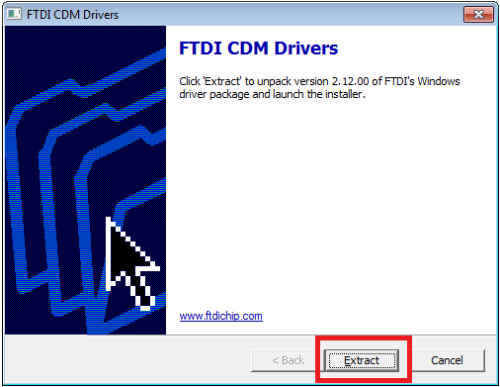
\includegraphics[width=6 cm]{figuras/instalacion7.png}\\
\caption{Instalador de drivers FTDI parte 1.}
\label{driversFTDI}
\end{figure}
\begin{figure}[H]
\centering
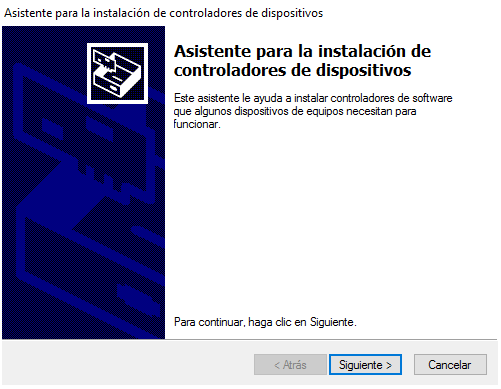
\includegraphics[width=5 cm]{figuras/instalacion8.png}\\
\caption{Instalador de drivers FTDI parte 2.}
\label{Fig10}
\end{figure}
\begin{figure}[H]
\centering
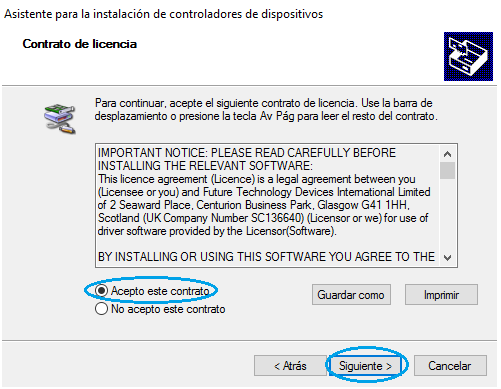
\includegraphics[width=6 cm]{figuras/instalacion9.png}\\
\caption{Instalador de drivers FTDI parte 3.}
\label{Fig11}
\end{figure}
\begin{figure}[H]
\centering
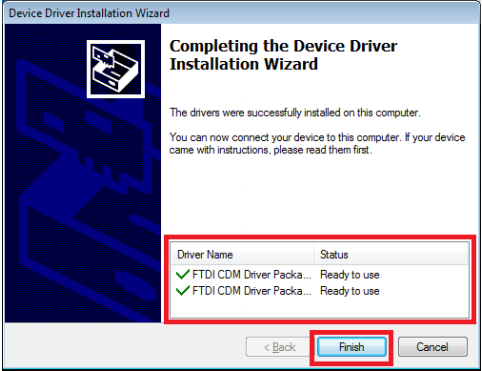
\includegraphics[width=6 cm]{figuras/instalacion10.png}\\
\caption{Instalador de drivers FTDI parte 4.}
\label{Fig12}
\end{figure}
\end{enumerate}
\item[•]\textbf{Paso 6}: Una posible falla que pueden surgir en esta instalación, es que puede presentarse un error en la comunicación a través del puerto virtual FTDI, que impide la correcta comunicación entre la placa y el entorno IDE. Su corrección debe efectuarse manualmente fuera del instalador, y es posible la aparición de una ventana de error emergente como la que se muestra en la Figura \ref{Fig13}.
\begin{figure}[!h]
\centering
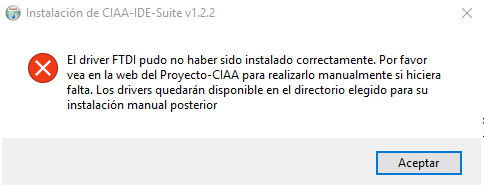
\includegraphics[width=9 cm]{figuras/instalacion11.png}\\
\caption{Instalador de drivers FTDI parte 5.}
\label{Fig13}
\end{figure}

\item[•]\textbf{Paso 7}: El instalador incluye en la carpeta donde se instaló el software (Por defecto C:/CIAA) un programa que configura el driver del controlador serie, emulado por la placa, para que uno de ellos pueda ser utilizado como interfaz JTAG. Dicho programa se llama $ Zadig\_Win\_7\_2\_1\_1.exe $, la Figura \ref{Fig14} muestra la ubicación del programa.
\begin{figure}[!h]
\centering
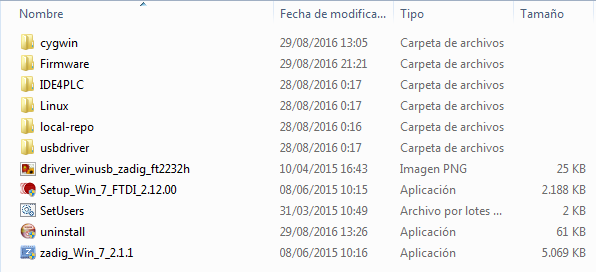
\includegraphics[width=6 cm]{figuras/instalacion12.png}\\
\caption{Instalador de drivers FTDI parte 6}
\label{Fig14}
\end{figure}

\item[•]\textbf{Paso 8}: Al abrir la aplicación, se presenta la Figura \ref{Fig15}. Antes de proceder, el usuario debe conectar la placa, posteriormente, debe abrir el menú contextual \textit{Options} y presionar sobre \textit{List all devices}
\begin{figure}[!h]
\centering
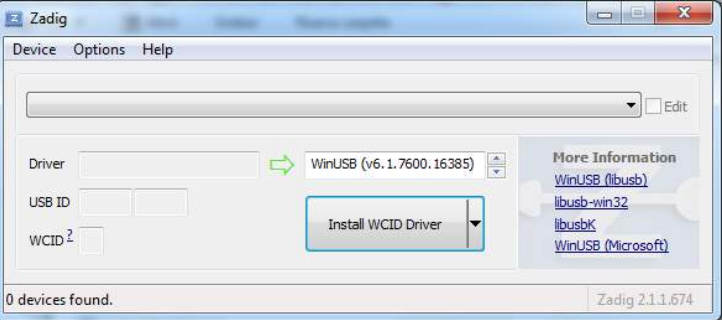
\includegraphics[width=6 cm]{figuras/instalacion13.png}\\
\caption{Entorno del software corrector Zadig para Windows.}
\label{Fig15}
\end{figure}

\item[•]\textbf{Paso 9}: Aparecerá una lista de dispositivos de comunicación relacionados al USB. Se tiene que buscar aquellos cuyos nombres tengan relación con el puerto serie (puede aparecer Dual RS232-HS, USB Serial Converter, o algo similar). Por lo general, aparecerán 2 con el mismo nombre, excepto que uno es Interface 0 y el otro Interface 1, como se muestra en la Figura \ref{Fig16} (la lista de drivers que se muestra puede diferir, dependiendo de la computadora que se utilice).

\begin{figure}[!h]
\centering
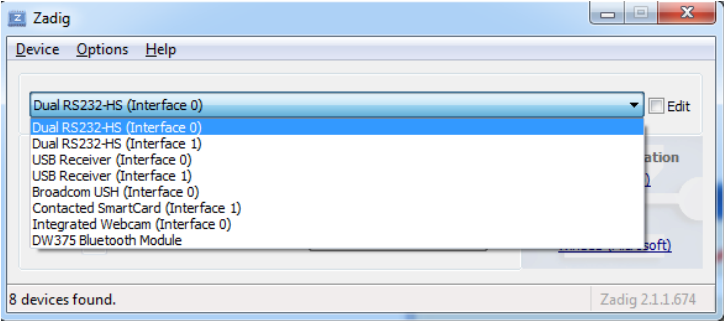
\includegraphics[width=8 cm]{figuras/instalacion14.png}\\
\caption{Lista de dispositivos vinculados a USB.}
\label{Fig16}
\end{figure}

\item[•]\textbf{Paso 10}: Para configurar el driver:

\begin{enumerate}
\item[•]Seleccionar la \textbf{Interfase 0}.
\item[•]Elegir el \textbf{“WinUSB v6.1”}.
\item[•]Hacer click en el botón \textbf{“Replace Driver”}.
\end{enumerate}
La Figura \ref{Fig17} muestra la ventana ya configurada:


\begin{figure}[H]
\centering
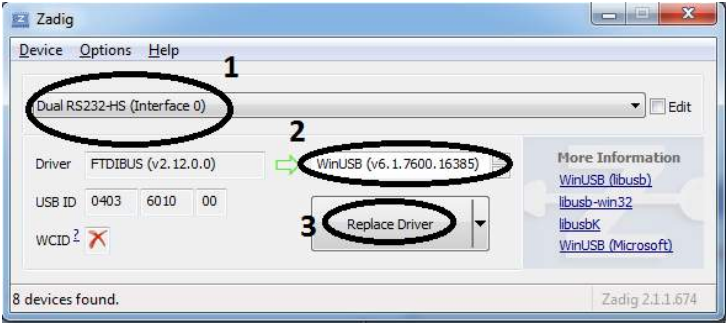
\includegraphics[width=13 cm]{figuras/instalacion15.png}\\
\caption{Configuración del Zadig para el reemplazo del driver}
\label{Fig17}
\end{figure}

\end{enumerate}



\section{Desinstalación}
Si se instaló el Software de CIAA-IDE y luego se desea desinstalarlo, se debe tener especial
cuidado en quitar cualquier contenido que se quiera conservar de la carpeta C:$\setminus$CIAA, o el directorio de instalación elegido. Esto se debe a que el desinstalador del Software CIAA-IDE elimina el directorio y todo su contenido.
\begin{enumerate}
\item[•]\textbf{Paso 1}: Ejecutar el programa \textit{uninstall.exe} ubicado en el directorio de instalación del programa.
\item[•]\textbf{Paso 2}: Luego se presenta la ventana de la Figura \ref{des1}. Hacer click en \textit{Siguiente}.
\begin{figure}[H]
\centering
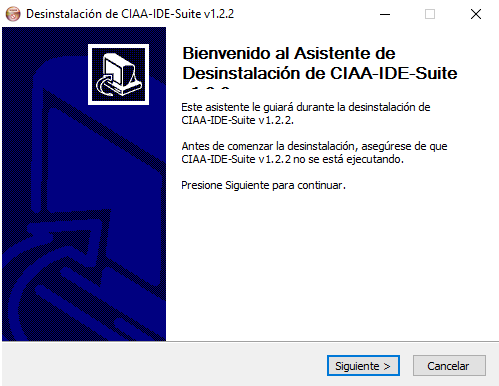
\includegraphics[width=8 cm]{figuras/des1.png}\\
\caption{Desinstalación del programa.}
\label{des1}
\end{figure}
\item[•]\textbf{Paso 3}: Seleccionar el directorio de instalación, en caso de haber instalado el programa en el directorio por defecto se tiene una ventana similar a la Figura \ref{des2}. Luego hacer click sobre \textit{Desinstalar}.
\begin{figure}[H]
\centering
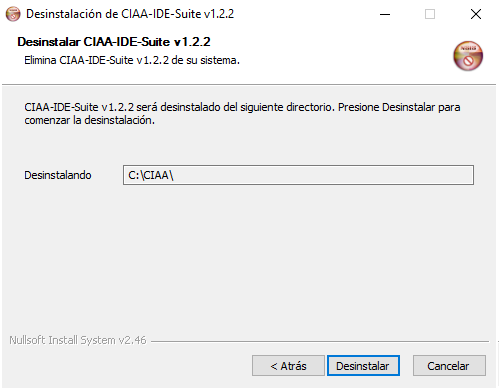
\includegraphics[width=8 cm]{figuras/des2.png}\\
\caption{Desinstalación del programa.}
\label{des2}
\end{figure}
\item[•]\textbf{Paso 4}: Finalmente se presenta una ventana como la Figura \ref{des3}. Sobre ella debe hacer click sobre \textit{Terminar}.
\begin{figure}[H]
\centering
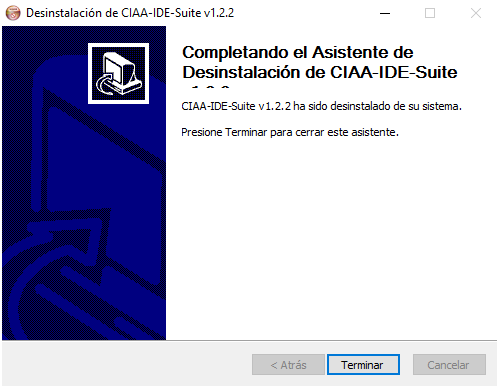
\includegraphics[width=8 cm]{figuras/des3.png}\\
\caption{Desinstalación del programa.}
\label{des3}
\end{figure}
\end{enumerate}
\section{Primeros Pasos con la EDU-CIAA}

\subsection{Programacion en Baremetal a través de libreria sAPI}\label{sec:programacionbaremetal}
La programación en Baremetal se refiere a la realizada cuando no se incluye un Sistema Operativo. Debido a que la programación de la placa en Baremetal puede tornarse un tanto engorrosa en principio, es posible utilizar una biblioteca, llamada \textit{sAPI}, diseñada para la implementación de proyectos en Baremetal con la placa EDU CIAA. Esta biblioteca implementa una API simple para la programación de la placa. Una API es una interfaz de programación de aplicaciones, y consta de un conjunto de subrutinas, funciones y procedimientos (o métodos, en la programación orientada a objetos) para permitir ser utilizada por otro software como una capa de abstracción en la programación (aunque no necesariamente) entre los niveles o capas inferiores y las superiores del software.
 \\
 
La motivación para el desarrollo de la biblioteca sAPI surge de la necesidad de manejar los periféricos directamente desde una máquina virtual de Java para el desarrollo de Java sobre la CIAA y corresponde a la parte de bajo nivel de las clases de periféricos en Java que básicamente bindea a funciones escritas en C.
Luego se extendió la misma para facilitar el uso de la EDU-CIAA-NXP a personas no expertas en la arquitectura del LPC4337 facilitando el uso de esta plataforma.
 \\
 
La idea es tener periféricos abstractos y lo más genéricos posibles. Que sea bien independiente de la arquitectura y en lo posible que las funciones sean todas del tipo:
\begin{enumerate}
\item[$\bullet$]	moduloConfig();
\item[$\bullet$]  moduloRead();
\item[$\bullet$]  moduloWrite();
\end{enumerate}

Los siguientes módulos estan incluidos:
\begin{enumerate}
\item[$\bullet$]Tipos de datos.
\item[$\bullet$]Mapa de periféricos.
\item[$\bullet$]Plataforma.
\item[$\bullet$]Tick.
\item[$\bullet$]Retardo.
\item[$\bullet$]E/S Digital.
\item[$\bullet$]E/S Analógica.
\item[$\bullet$]Uart.
\end{enumerate}   

Es necesario destacar que actualmente se encuentra disponible para las plataformas EDU CIAA NXP (microcontrolador NXP LPC4337) y para la plataforma CIAA NXP (microcontrolador NXP LPC4337). La Figura \ref{Fig18} ilustra como son las distintas capas de software y la correspondiente ubicación de la \textit{sAPI}.
\begin{figure}[H]
\centering
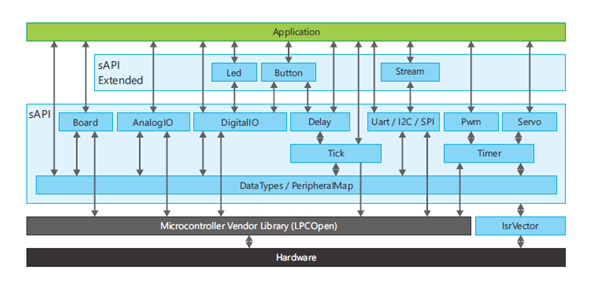
\includegraphics[width=12 cm]{figuras/primer_proy18.png}\\
\caption{Capas de abstracción de software}
\label{Fig18}
\end{figure} 

Breve descripcion de los modulos de la biblioteca:
\begin{enumerate}
\item[•]\textbf{sAPI$\_$Config}: Contiene configuraciones de la biblioteca.
\item[•]\textbf{sAPI$\_$DataTypes}: Define las siguientes constantes:
\begin{enumerate}
\item[•]Estados lógicos, \textit{TRUE} y \textit{FALSE}.
\item[•]Estados funcionales \textit{ON} y \textit{OFF}.
\item[•]Estados electricos \textit{HIGH} y \textit{LOW}.
\item[•]Tipos de datos: Booleanos (\textit{bool$\_$t}), enteros sin signo(\textit{uint8$\_$t, uint16$\_$t, uint32$\_$t, uint64$\_$t}), enteros con signo (\textit{int8$\_$t, int16$\_$t, int32$\_$t, int64$\_$t}).
\end{enumerate}
\item[•]\textbf{sAPI$\_$IsrVector}: Contiene la tabla de vectores de interrupción.
\item[•]\textbf{sAPI$\_$Board}: Contiene la función de configuración para inicialización de la plataforma de hardware.
\item[•]\textbf{sAPI$\_$PeripheralMap}: Contiene el mapa de periféricos, para la interpretación de éste, el usuario debe utilizar el diagrama esquemático de la placa y el archivo \textit{PeripheralMap$.txt$} ubicado sobre el directorio \textit{sapi-bm}.
\item[•]\textbf{sAPI$\_$DigitalIO}: Utilizada para el manejo de entradas y salidas digitales.
\end{enumerate}


Utilización de biblioteca sAPI:
\begin{enumerate}
\item[•]Descargar la version más reciente de dicha biblioteca, a traves del repositorio de la misma, ubicado en la pagina web.
\item[•]Luego de haber descargado la versión actual de  sAPI se procede a copiar la carpeta \textit{sapi$\_$bm} y pegarla en \textit{C$:/$CIAA$/$Firmware$/$modules}. La Figura \ref{sapiuso} ilustra este proceso.
\begin{figure}[H]
\centering
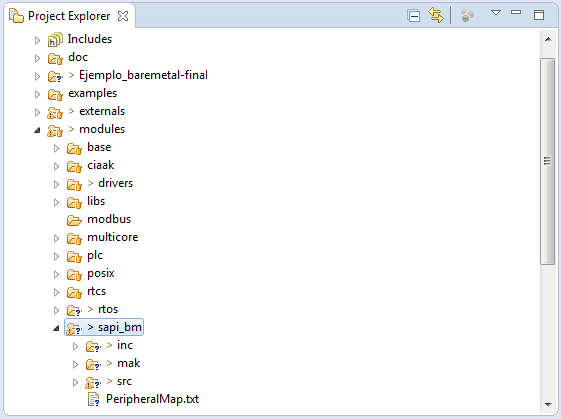
\includegraphics[width=8 cm]{figuras/sapiuso.png}\\
\caption{Ubicación de módulo \textit{sAPI}.}
\label{sapiuso}
\end{figure} 
\item[•]Al utilizar la biblioteca \textit{sAPI} para un proyecto en Baremetal, se debe modificar el makefile del mismo dentro de la carpeta mak y cambiar la última línea de: \textbf{MODS += externals \$(DS)drivers}, y reemplazarla por:  \textbf{MODS += modules \$ (DS)sapi$\_$bm}.
\item[•]Luego, sobre cada archivo fuente en la que se ejecuten instrucciones que contenga esta biblieteca, se debe realizar la inclusión del mismo mediante la instruccion: \textbf{\# include “sAPI.h”}.Debe aclararse que en la versión 0.3.0 no es necesario incluir el archivo \textit{chip.h}.
\item[•]Para la compilación y depuración del programa mediante el IDE del Firmware, se debe colocar sobre la carpeta Firmware y mediante click derecho, el usuario debe ubicarse en \textit{Propiedades}$\rightarrow$\textit{C/C++ Build}$\rightarrow$\textit{Behaviour}. A continuación debe modificar sobre la rama \textit{Clean}, y reemplazar la palabra \textit{Clean\_ generate} por  \textit{clean}, como puede apreciarse en la Figura \ref{Fig19}.
\begin{figure}[H]
\centering
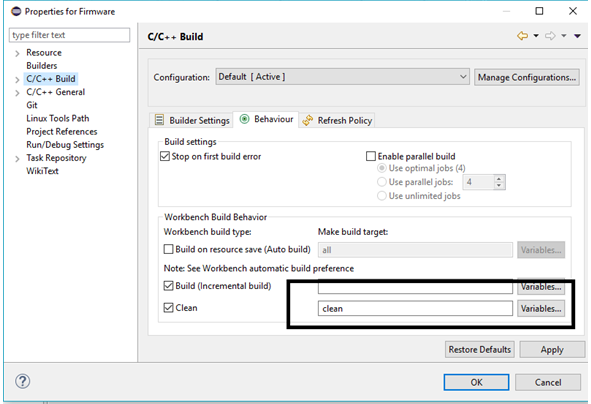
\includegraphics[width=8 cm]{figuras/f1.png}\\
\caption{Cambio de “clean$\_$generate” a “clean”.}
\label{Fig19}
\end{figure}


\end{enumerate}

\subsection{Implementación de ejemplo N$^{\circ}$1: Salidas Digitales}\label{sec:ej1sapi}
El primer ejemplo aborda las salidas digitales, a través de los leds que provee la placa EDUCIAA. Este programa enciende los leds de la placa en forma secuencial, de izquierda a la derecha. Luego de finalizar esta secuencia, se apagan de derecha a izquierda.
\begin{enumerate}
\item[•]\textbf{Paso 1}: Sobre el IDE de la placa, debe agregarse un nuevo directorio, realizando click derecho sobre \textit{Firmware}, luego se selecciona la opción \textit{New} $\rightarrow$ \textit{Folder}. La Figura \ref{nuevodirectorio} ilustra lo explicado.
\begin{figure}[H]
\centering
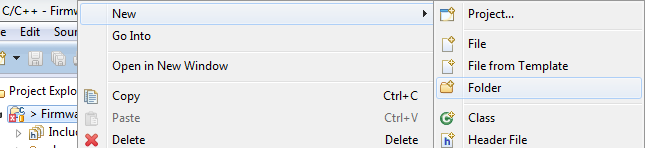
\includegraphics[width=8 cm]{figuras/f43.png}
\caption{Creacion de Nuevo Directorio.}
\label{nuevodirectorio}
\end{figure}
\item[•]\textbf{Paso 2}: A continuación se abre una ventana como la que se muestra en la Figura \ref{nuevodirectorio2}, que permite designar el nombre del directorio donde se ubica el proyecto que se quiere implementar. El usuario debe recordar que para compilar dicho proyecto debe establecer la ruta que le corresponde sobre el archivo \textit{Makefile}. Asimismo, deben agregarse los directorios \textit{etc}, \textit{mak}, \textit{inc}, y \textit{src}, sobre el directorio creado recientemente.
\begin{figure}[H]
\centering
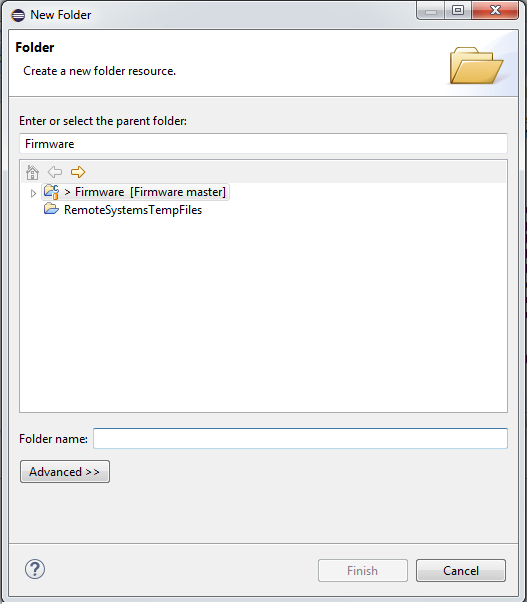
\includegraphics[width=8 cm]{figuras/f44.png}
\caption{Creación de Nuevo Directorio.Ventana de Creación.}
\label{nuevodirectorio2}
\end{figure}

 
Para generar el archivo cabecera, el usuario debe ubicarse sobre la carpeta \textit{inc}, y luego oprimiendo click derecho, debe seleccionar la opción \textit{New} $\rightarrow$ \textit{Header File}. A continuación se abre una ventana cuyo aspecto es similar al de la Figura \ref{archivocabecerasapi1}.
\begin{figure}[H]
\centering
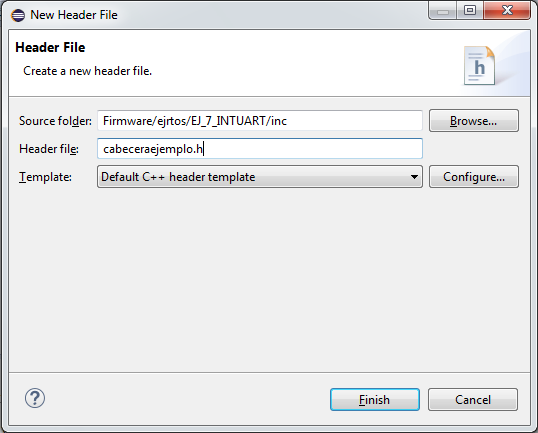
\includegraphics[width=8 cm]{figuras/f27.png}
\caption{Generación de archivo cabecera para implementación de proyecto.}
\label{archivocabecerasapi1}
\end{figure}
En ella, se debe establecer el nombre del archivo cabecera. Al terminar la escritura de su nombre, debe escribirse la terminación \textit{.h}, y oprimir el boton \textit{Finish}, para concluir la generacion de dicho archivo.
En este caso, el archivo cabecera se define como \textit{Ejemplo$\_$1.h}.

\item[•]\textbf{Paso 3}: Para generar el archivo fuente, el usuario debe ubicarse sobre la carpeta \textit{inc}, y luego oprimiendo click derecho, debe seleccionar la opción \textit{New} $\rightarrow$ \textit{Source File}. A continuación se abre una ventana cuyo aspecto es similar al de la Figura \ref{archivofuentesapi1}, en ella, se debe establecer el nombre del archivo fuente, el cual en este caso es \textit{Ejemplo$\_$1.c}. Al terminar la escritura de su nombre, debe escribirse la terminación \textit{.c}, y oprimir el boton \textit{Finish}, para concluir la generacion de dicho archivo.
\begin{figure}[!h]
\centering
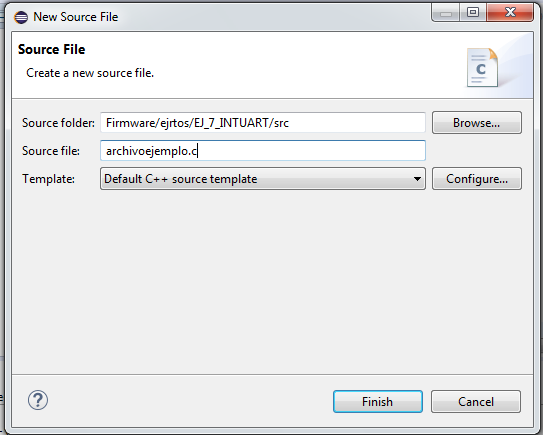
\includegraphics[width=8 cm]{figuras/f28.png}
\caption{Generación de archivo fuente para implementación de proyecto.}
\label{archivofuentesapi1}
\end{figure}
\item[•]\textbf{Paso 4}: Ingresar el archivo cabecera de la librería \textit{sAPI} para poder referenciar los módulos a utilizar y referenciar el archivo cabecera del proyecto en caso de que el usuario desee declarar de forma directa alguna función o algún identificador. La Figura \ref{inclusionsapi1} ilustra dicho concepto.

\begin{figure}[!h]
\centering
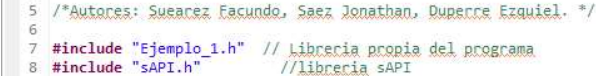
\includegraphics[width=5 cm]{figuras/f2.png}
\caption{Generación de archivo fuente para implementación de proyecto.}
\label{inclusionsapi1}
\end{figure}

\item[•]\textbf{Paso 5}: Una vez declarada la función principal \textit{main()}, es importante destacar algunas funciones utilizadas:
\begin{enumerate}
\item[•]\textit{boardconfig()}: Esta función se encarga de la configuración para inicializar la plataforma del hardware. No se debe especificar ningún parámetro.
\item[•]\textit{tickconfig(A,B)}: Configura una interrupción periódica de temporizador cada tickRateMSvalue milisegundos para utilizar de base de tiempo del sistema. El parámetro A es el tiempo en milisegundos en el que se desee interrumpir el periférico Systick y aumente un contador que se usa para el módulo delay o para lo que se requiera. Sobre el parámetro B se especifica la función a ejecutar en cada tick.
\item[•]\textit{digitalConfig(A,B)}: Inicializa los puertos GPIO de la placa y define sus funciones como entradas y salidas digitales. El parametro A debe ser 0, mientras que el parámetro B debe ser \textit{ENABLE$\_$DIGITAL$\_$IO}.
\item[•]\textit{digitalWrite(A,B)}: Permite el establecimiento en \textit{ALTO} o en \textit{BAJO} de un pin configurado como salida digital. Sobre el parámetro A de la funcion debe establecerse el nombre del PIN, teniendo en cuenta la definición realizada sobre el módulo \textit{sAPI$\_$PeripheralMap}. Sobre el parámetro B debe determinarse es el estado funcional \textit{ON} u \textit{OFF}.
\item[•]\textit{delay(A)}: Permite implementar una temporización en ms sobre el parámetro A de dicha función.
\end{enumerate}
\item[•]\textbf{Paso 6}: Ingresar el código \textit{Ejemplo$\_$1.c} ubicado en la carpeta \textit{EJ$\_$1$\_$BM}. 
\item[•]\textbf{Paso 7}:Para realizar la compilación debe seleccionarse el directorio \textit{Firmware} y posteriormente hacer click sobre el botón \textit{Build}.
\end{enumerate}
\subsection{Implementación de ejemplo N$^{\circ}$2: Entradas y Salidas Digitales}\label{sec:ej2sapi}

El siguiente ejemplo tiene como objetivo el manejo de las entradas y salidas digitales, dicho programa enciende los leds incorporados sobre la placa, de acuerdo con la cantidad de veces que se oprime la tecla \textit{TEC1}. Sobre dicho ejemplo se implementó una maquina de estado, a través del programa \textit{uModel Factory} para poder establecer un orden sobre los eventos y las acciones que debe ejecutar el microcontrolador.
 \\
 
Debe tenerse en cuenta que se implementan multiples archivos fuentes y cabeceras, en particular, el archivo fuente \textit{funciones.c} define las acciones y la evaluación de los eventos y \textit{funciones.h} establece la declaración de dichas funciones y de los estados.
 \\
 
La Figura \ref{tablatransicionej2} especifica la Tabla de Transiciónes de la MEF.
\begin{figure}[H]
\centering
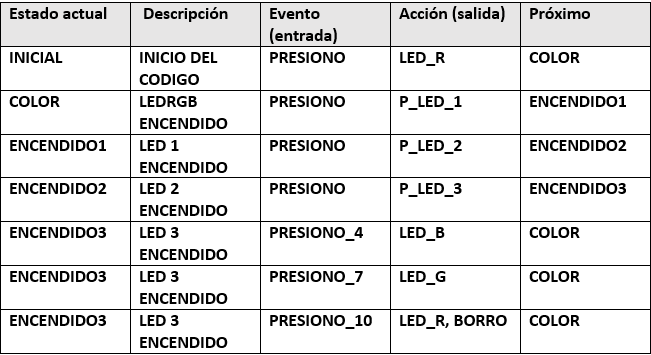
\includegraphics[width=10 cm]{figuras/f45.png}\\
\caption{Tabla de Transiciónes de N$^{\circ}$2.}
\label{tablatransicionej2}
\end{figure}
La Figura \ref{Fig22} especifica el diagrama de estados del ejemplo:

\begin{figure}[H]
\centering
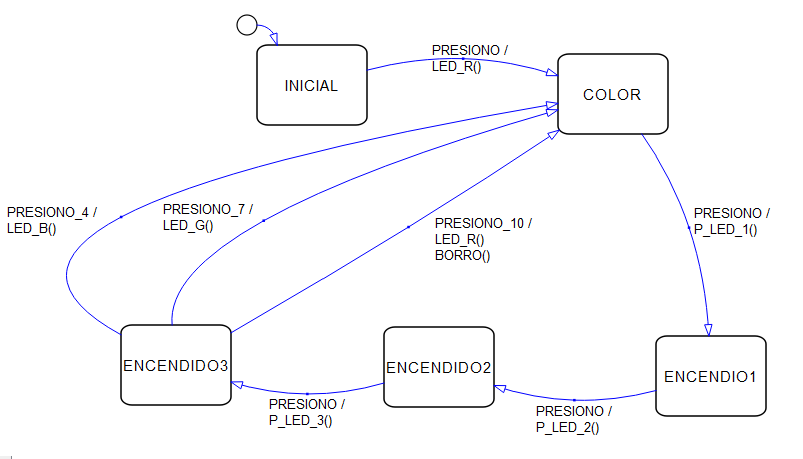
\includegraphics[width=10 cm]{figuras/f4.png}\\
\caption{Diagrama de estados de ejemplo N$^{\circ}$2.}
\label{Fig22}
\end{figure}

La funcion \textit{digitalRead(A)} permite determinar el estado funcional de un pin configurado como entrada digital, sobre el parámetro A debe determinarse el nombre del pin sobre el cual se desea efectuar la lectura. Debe tenerse en cuenta que dicho nombre debe corresponder al que se encuentra definido sobre el módulo \textit{sAPI$\_$PeripheralMap.h}.

\begin{enumerate}
\item[•]\textbf{Paso 1}: Realizar la generación de los archivos cabecera y fuente como se establecen en los Pasos 1, 2 y 3 sobre la seccion \ref{sec:ej1sapi}.

\item[•]\textbf{Paso 2}: Realizar la generación de los archivos cabecera \textit{funciones.h} y archivos fuente \textit{funciones.c} de la misma forma que que el paso anterior.

\item[•]\textbf{Paso 3}: Ingresar sobre el archivo cabecera creado en el paso anterior, el código que contiene el archivo \textit{funciones.h}, ubicado sobre la carpeta \textit{EJ$\_$2$\_$BM}.

\item[•]\textbf{Paso 4}: Ingresar sobre el archivo fuente creado en el paso anterior, el código que contiene el archivo \textit{funciones.c}, ubicado sobre la carpeta \textit{EJ$\_$2$\_$BM}.

\item[•]\textbf{Paso 5}: Ingresar sobre el archivo fuente creado en el paso 1, el código que contiene el archivo \textit{Ejemplo$\_$2.c}, ubicado sobre la carpeta \textit{EJ$\_$2$\_$BM}.

\item[•]\textbf{Paso 6}: Realizar la compilación y depuración del programa.
\end{enumerate}



\subsection{Implementación de ejemplo N$^{\circ}$3: Entradas Analógicas y Uso de Display 7 Segmentos}\label{sec:ej3sapi}
En este ejemplo se realizan dos tareas distintas, dependiendo de la tecla pulsada (\textit{TEC1} y \textit{TEC2}). Si se pulsa la tecla \textit{TEC1}, se encienden los leds en una secuencia determinada. Mientras que si se pulsa la tecla \textit{TEC2}, se realiza una muestra de los dígitos desde 1 hasta 9 a través del Display 7 Segmentos. 
 \\
 
Se implementa una maquina de estados en donde se establecen los prototipos de funciones que corresponden a los eventos y las acciones que acontecen. 
La Figura \ref{tablatransicionej3} especifica la Tabla de Transiciónes de la MEF.
\begin{figure}[H]
\centering
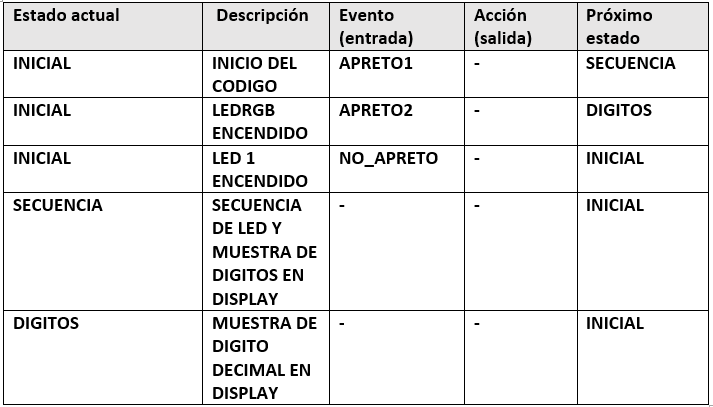
\includegraphics[width=10 cm]{figuras/IMAGEN-EJEMPLO3.png}\\
\caption{Tabla de Transiciónes de N$^{\circ}$3.}
\label{tablatransicionej3}
\end{figure}

La Figura \ref{diagramaej3} especifica el diagrama de estados del ejemplo:

\begin{figure}[H]
\centering
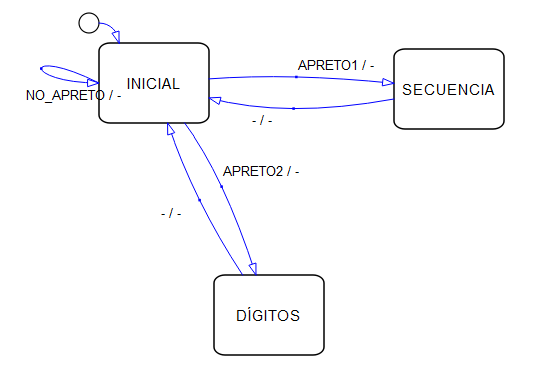
\includegraphics[width=8 cm]{figuras/ejemplo-3.png}\\
\caption{Diagrama de estados de ejemplo N$^{\circ}$3.}
\label{diagramaej3}
\end{figure}
Para el manejo del display se utiliza una biblioteca. Para ello, deben generarse dos archivos los cuales pertenecen a la cabecera y a la fuente de dicha librería. Sobre la cabecera deben establecerse las inclusiones de la librería \textit{sAPI} y las declaraciones de las funciones que corresponden con el manejo del dispositivo.
 \\
 
En este tutorial se realiza el manejo de un display de 7 segmentos del tipo cátodo común, de manera que para provocar el encendido de un led perteneciente al arreglo, se debe establecer en alto la salida de el pin conectado a dicho led. La librería que provee este tutorial determina el conexionado de los pines del display, sobre los correspondientes terminales GPIO ubicados en la placa EDU CIAA. La Figura \ref{Fig23} ilustra los terminales de la placa y del display utilizados para la conexión del dispositivo.


\begin{figure}[H]
\centering
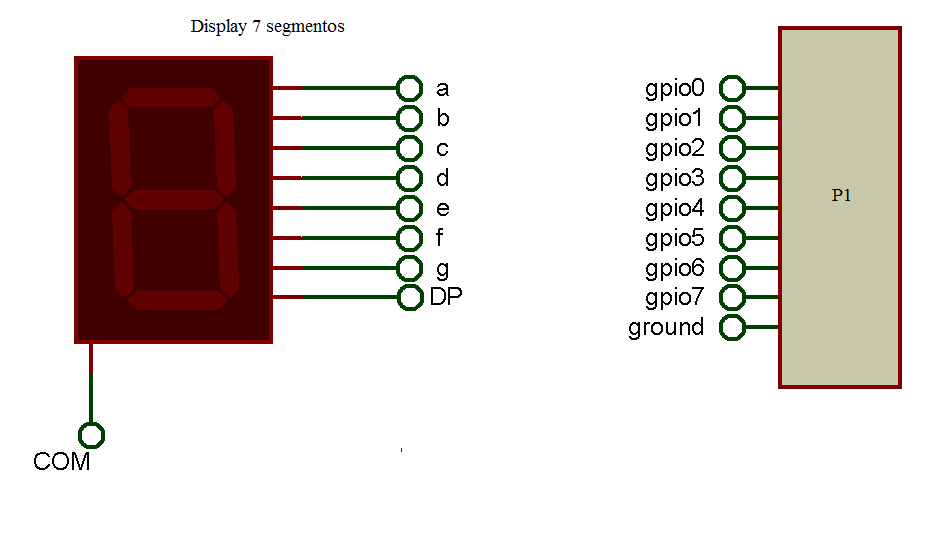
\includegraphics[width=12 cm]{figuras/dsp7seg.png}\\
\caption{Diagrama de conexión Display 7 Segmentos.}
\label{Fig23}
\end{figure}

\underline{Uso de Entradas Analógicas}:

En este código se hará uso del conversor analógico digital que posee esta placa. La idea es introducir una tensión analógica mediante la entrada CH1 y luego convertirla en un valor digital, para que posteriormente dentro del código, mediante operaciones matemáticas, poder mostrar dicho valor por el display.
 \\
 
La instrucción que implementa la biblioteca \textit{sAPI} para la lectura analógica es \textit{analogRead()}, sobre dicha función no debe especificarse ningún parámetro de entrada, sin embargo, debe tenerse en cuenta que retorna un valor de salida, el cual debe almacenarse sobre una variable del tipo \textit{uint16$\_$t}.

\begin{enumerate}
\item[•]\textbf{Paso 1}: Realizar la generación de los archivos cabecera y fuente como se establecen en los Pasos 1, 2 y 3 sobre la seccion \ref{sec:ej1sapi}.

\item[•]\textbf{Paso 2}: Realizar la generación de los archivos cabecera \textit{funciones.h} y archivos fuente \textit{funciones.c} de la misma forma que que el paso anterior.

\item[•]\textbf{Paso 3}: Ingresar sobre el archivo cabecera creado en el paso anterior, el código que contiene el archivo \textit{funciones.h}, ubicado sobre la carpeta \textit{EJ$\_$3$\_$BM}.

\item[•]\textbf{Paso 4}: Ingresar sobre el archivo fuente creado en el paso anterior, el código que contiene el archivo \textit{funciones.c}, ubicado sobre la carpeta \textit{EJ$\_$3$\_$BM}.

\item[•]\textbf{Paso 5}: Ingresar sobre el archivo fuente creado en el paso 1, el código que contiene el archivo \textit{Ejemplo$\_$3.c}, ubicado sobre la carpeta \textit{EJ$\_$3$\_$BM}.

\item[•]\textbf{Paso 6}: Realizar la compilación y depuración del programa.
\end{enumerate}

\subsection{Implementación de ejemplo N$^{\circ}$4: Conversor Digital/Analógico (DAC)}\label{sec:ej4sapi}
%\label{sec:dac}

Un convertidor Digital/Analógico (DAC), es un dispositivo electrónico que recibe como dato de entrada un valor digital (en forma de una palabra de "n" bits) y lo transforma a una señal analógica. Cada una de las combinaciones binarias de entrada es convertida en niveles lógicos de tensión de salida. Un DAC transfiere información expresada en forma digital a una forma analógica. Para ubicar la función de este dispositivo conviene recordar que un sistema combina y relaciona diversos subsistemas que trabajan diferentes con tipos de información analógica, como son: Magnitudes eléctricas, mecánicas, etc.
 \\
 
El siguiente ejemplo muestra al usuario como realizar el uso del módulo ADC de la placa, para realizar la lectura de una entrada analógica. Este programa enciende algunos de los leds de la placa, en función a la magnitud de la tensión leída. Por ejemplo, si la tensión leída es 2[V], entonces se encienden dos leds.
 \\
 
La placa EDU-CIAA posee un DAC de 10 bits de resolución ,por lo tanto,el número de niveles de voltaje de salida analógico que es capaz de generar es de $2^{n}=2^{10}=1024$.
Para la implementación del ejemplo, es posible realizar la lectura del terminal medio de un potenciómetro, la Figura \ref{Fig24} ilustra la conexión realizada. Debe tenerse en cuenta que es posible realizar la conexión del potenciómetro a partir de la terminal de 5[V] y la terminal GNDA que ofrece la placa.

\begin{figure}[H]
\centering
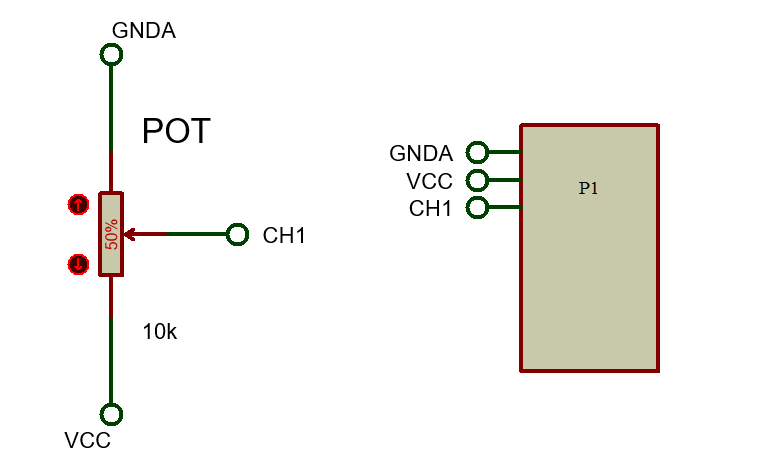
\includegraphics[width=10 cm]{figuras/potenciometro_ejemplo_4_baremetal.png}\\
\caption{Diagrama de conexión potenciómetro para lectura analógica.}
\label{Fig24}
\end{figure}

Este ejemplo utiliza maquinas de estado para poder establecer un orden sobre los eventos y las acciones que debe ejecutar el microcontrolador.
La Figura \ref{tablatransicionej4} especifica la Tabla de Transiciónes de la MEF.
\begin{figure}[H]
\centering
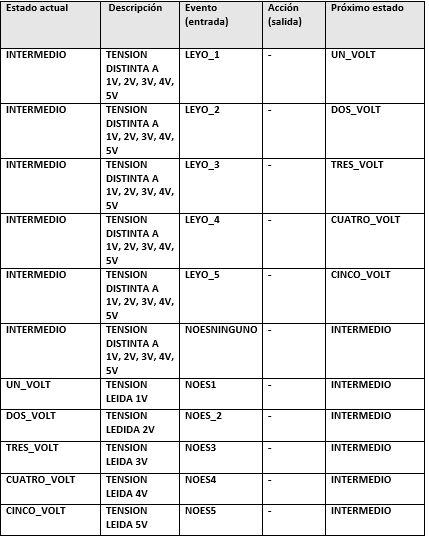
\includegraphics[width=8 cm]{figuras/IMAGEN-EJEMPLO4.png}\\
\caption{Tabla de Transiciónes de N$^{\circ}$4.}
\label{tablatransicionej4}
\end{figure}
La Figura \ref{diagramaej4} especifica el diagrama de estados del ejemplo:

\begin{figure}[H]
\centering
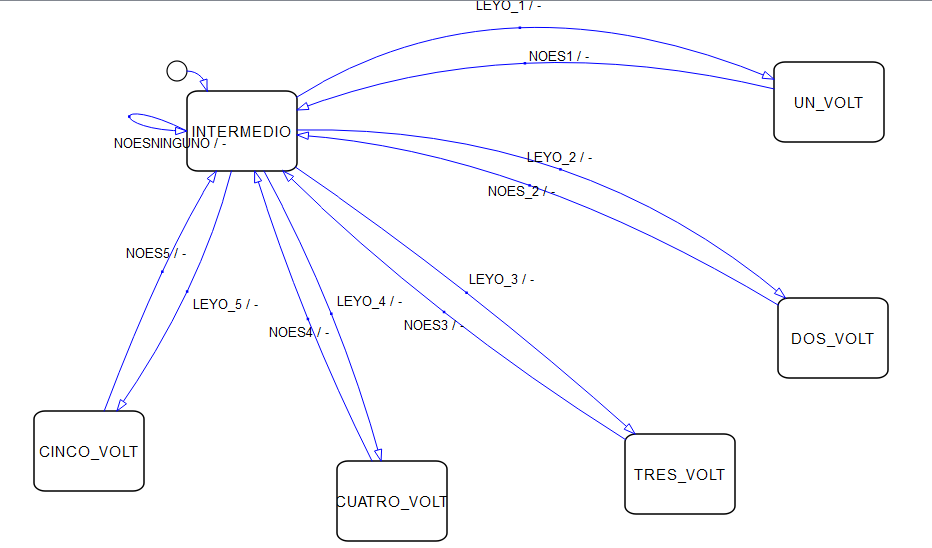
\includegraphics[width=8 cm]{figuras/ejemplo-4.png}\\
\caption{Diagrama de estados de ejemplo N$^{\circ}$4.}
\label{diagramaej4}
\end{figure}
La instrucción \textit{analogConfig( ENABLE$\_$ANALOG$\_$INPUTS )} se encarga de habilitar las entradas analógicas. Mientras que \textit{analogConfig( ENABLE$\_$ANALOG$\_$OUTPUTS )} se encarga de habilitar las salidas analógicas, con las que trabajara el DAC.

\begin{enumerate}
\item[•]\textbf{Paso 1}: Realizar la generación de los archivos cabecera y fuente como se establecen en los Pasos 1, 2 y 3 sobre la seccion \ref{sec:ej1sapi}.

\item[•]\textbf{Paso 2}: Realizar la generación de los archivos cabecera \textit{funciones.h} y archivos fuente \textit{funciones.c} de la misma forma que que el paso anterior.

\item[•]\textbf{Paso 3}: Ingresar sobre el archivo cabecera creado en el paso anterior, el código que contiene el archivo \textit{funciones.h}, ubicado sobre la carpeta \textit{EJ$\_$4$\_$BM}.

\item[•]\textbf{Paso 4}: Ingresar sobre el archivo fuente creado en el paso anterior, el código que contiene el archivo \textit{funciones.c}, ubicado sobre la carpeta \textit{EJ$\_$4$\_$BM}.

\item[•]\textbf{Paso 5}: Ingresar sobre el archivo fuente creado en el paso 1, el código que contiene el archivo \textit{Ejemplo$\_$4.c}, ubicado sobre la carpeta \textit{EJ$\_$4$\_$BM}.

\item[•]\textbf{Paso 6}: Realizar la compilación y depuración del programa.
\end{enumerate}


\subsection{Implementación de ejemplo N$^{\circ}$5: Uso de UART y Display LCD 16x2}\label{sec:ej5sapi}
En este código se utiliza el modulo conversor analógico digital de la placa, para efectuar la lectura de una entrada analógica sobre esta. En el caso que dicha medición sea superior a 2[V], se establece una salida analógica de 2[V] utilizando el módulo conversor digital analógico. De forma similar, si la tensión de entrada resulta mayor a 4[V], se define una salida analógica de 3[V].
Es necesario destacar que la placa ya integra internamente el conversor digital analógico, de modo que no es necesario realizar una interfaz para la ejecución de dicha salida, además, es necesario destacar que la tensión de referencia interna se encuentra establecida, y adquiere un valor igual a 3.3[V]. La Figura \ref{Fig26} ilustra el esquemático que muestra dicho concepto.


\begin{figure}[H]
\centering
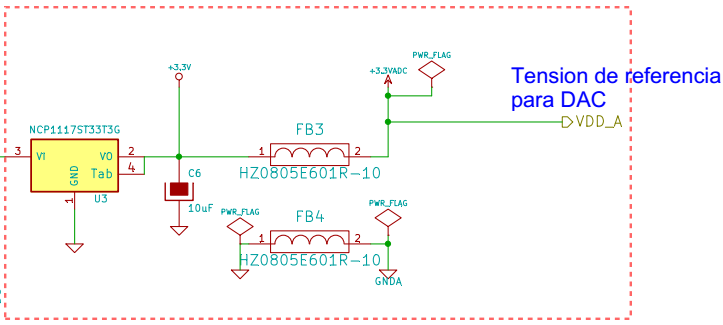
\includegraphics[width=10 cm]{figuras/f8.png}\\
\caption{Ilustración de tensión de referencia de DAC.}
\label{Fig26}
\end{figure}


La instrucción \textit{analogRead()}, permite realizar la lectura de la tensión aplicada sobre el canal 1 del modulo ADC0 de la placa. A partir de la conversión a tensión, el programa aplica la tensión de salida correspondiente.
 \\
 
Este ejemplo también utiliza maquina de estado para establecer un orden sobre los eventos y las acciones que debe ejecutar el microcontrolador. La Figura \ref{tablatransicionej5} especifica la Tabla de Transiciónes de la MEF.
\begin{figure}[H]
\centering
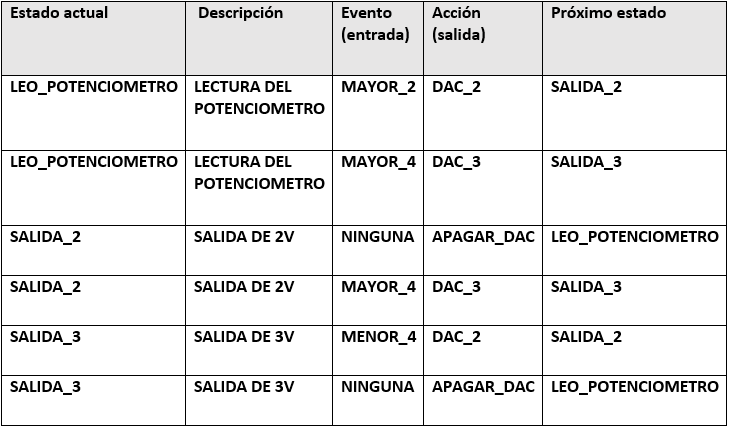
\includegraphics[width=10 cm]{figuras/IMAGEN-EJEMPLO5.png}\\
\caption{Tabla de Transiciónes de N$^{\circ}$5.}
\label{tablatransicionej5}
\end{figure}

La Figura \ref{diagramaej5} especifica el diagrama de estados del ejemplo:

\begin{figure}[H]
\centering
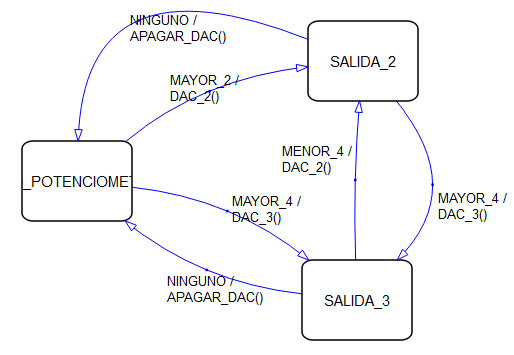
\includegraphics[width=10 cm]{figuras/f10.png}\\
\caption{Diagrama de estados de ejemplo N$^{\circ}$5.}
\label{diagramaej5}
\end{figure}

\begin{enumerate}
\item[•]\textbf{Paso 1}: Realizar la generación de los archivos cabecera y fuente como se establecen en los Pasos 1, 2 y 3 sobre la seccion \ref{sec:ej1sapi}.

\item[•]\textbf{Paso 2}: Realizar la generación de los archivos cabecera \textit{funciones.h} y archivos fuente \textit{funciones.c} de la misma forma que que el paso anterior.

\item[•]\textbf{Paso 3}: Ingresar sobre el archivo cabecera creado en el paso anterior, el código que contiene el archivo \textit{funciones.h}, ubicado sobre la carpeta \textit{EJ$\_$5$\_$BM}.

\item[•]\textbf{Paso 4}: Ingresar sobre el archivo fuente creado en el paso anterior, el código que contiene el archivo \textit{funciones.c}, ubicado sobre la carpeta \textit{EJ$\_$5$\_$BM}.

\item[•]\textbf{Paso 5}: Ingresar sobre el archivo fuente creado en el paso 1, el código que contiene el archivo \textit{Ejemplo$\_$5.c}, ubicado sobre la carpeta \textit{EJ$\_$5$\_$BM}.

\item[•]\textbf{Paso 6}: Realizar la compilación y depuración del programa.
\end{enumerate}




\subsection{Implementación de ejemplo N$^{\circ}$6: Comunicación Serial}\label{sec:serial}
El siguiente ejemplo introduce al usuario en la utilización de comunicación serial, es necesario destacar que para la implementación del ejemplo se utiliza el programa \textit{Octoplus Terminal} para la visualización y simulación del envío y transmisión de datos a través del terminal conectado sobre el puerto USB.
 \\
 
El programa se encuentra disponible de forma gratuita en la dirección web \textit{http://octoplus-terminal.software.informer.com/download/}. La instalación de dicho programa es simple, sin embargo, es necesario destacar que durante dicho proceso, el usuario debe obviar la instalación de los drivers que provee dicho programa.
 \\
 
Si bien ofrece distintas herramientas para la programación de sistemas embebidos, este tutorial se centra en la utilización de dicho programa para el envío y la recepción de datos sobre el terminal perteneciente a la placa. Para ello, a continuación se realizará una serie de pasos para la utilización de \textit{Octoplus} junto con la placa.
 \\
 
Es necesario mencionar que si existe un programa ya cargado previamente, también es posible utilizar \textit{Octoplus} de forma similar.
 \\
 
En este apartado se verá un código base para utilizar la UART del LPC4337 mediante las funciones que incluye la librería sAPI. Las funciones provistas por esta librería son las encargadas de realizar los siguientes pasos básicos para poder utilizar la UART0.

\begin{enumerate}
\item[•]Habilitar la alimentación del periférico.
\item[•]Habilitar el clock al periférico.
\item[•]Configurar la velocidad de transmisión.
\item[•]Habilitar las FIFO del transmisor y el receptor.
\item[•]Configurar la función de los pines para utilizarlo con la UART0.
\item[•]Habilitar la interrupción.
\end{enumerate}

El usuario debe seguir los siguientes pasos para implementar este ejemplo:
\begin{enumerate}
\item[•]\textbf{Paso 1}: Realizar la generación de los archivos cabecera y fuente como se establecen en los Pasos 1, 2 y 3 sobre la seccion \ref{sec:ej1sapi}.
\item[•]\textbf{Paso 2}: Suponiendo que el usuario ya se encuentran instalados los drivers para la placa, y las herramientas de depuración para la misma, luego de realizar la conexión entre la placa y la computadora a través de \textit{OpenOCD} (sobre la consola \textit{cygwin}), el usuario debe iniciar \textit{Octoplus}.
\item[•]\textbf{Paso 3}: A continuación se presenta una pantalla similar a la Figura \ref{Fig29}


\begin{figure}[H]
\centering
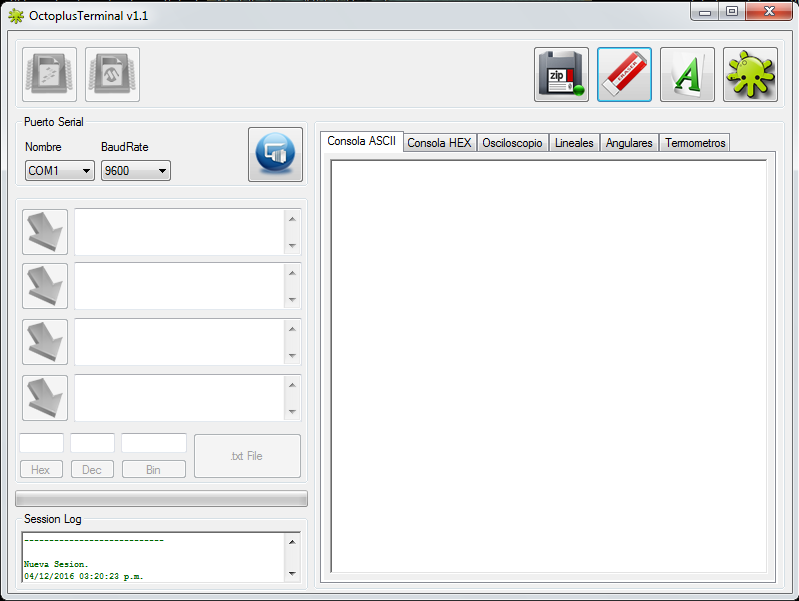
\includegraphics[width=6 cm]{figuras/f11.png}
\caption{Panel principal de \textit{Octoplus}.}
\label{Fig29}
\end{figure}


\item[•]\textbf{Paso 4}: Sobre la sección \textit{Puerto Serial} debe identificarse sobre el menú desplegable \textit{Nombre}, el puerto COM asociado a la placa. La Figura \ref{Fig30} ilustra dicho concepto


\begin{figure}[!h]
\centering
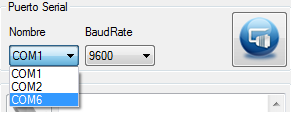
\includegraphics[width=4 cm]{figuras/f12.png}
\caption{Seleccion de puerto COM asociado a la placa.}
\label{Fig30}
\end{figure}

\item[•]\textbf{Paso 5}: Debe tenerse en cuenta sobre la instrucción \textit{uartConfig()}, perteneciente a la librería \textit{sAPI}, deben asignarse dos parámetros de entrada, uno de ellos indica el módulo de la UART sobre la cual se desea trabajar, en este caso el parámetro es \textit{UART$\_$USB}. El segundo parámetro que debe asignarse a dicha instrucción es la velocidad de transmisión en baudios. El valor de la velocidad previamente configurada sobre el programa debe ser configurado sobre el menú desplegable \textit{BaudRate}, ubicado sobre el costado derecho del menú desplegable \textit{Nombre}.Por ejemplo, si la velocidad configurada es igual a 9600 baudios, entonces sobre dicho menú debe seleccionarse 9600, como lo ilustra la Figura \ref{Fig30}.
\item[•]\textbf{Paso 6}: Al realizar la depuración, el usuario debe seleccionar el boton \textit{Abrir/Cerrar puerto COM}, el cual se encuentra sobre la derecha del menú desplegable \textit{BaudRate},como lo ilustra la Figura \ref{Fig29}.
\item[•]\textbf{Paso 7}: Para efectuar transmisiones sobre el puerto COM seleccionado, el usuario debe ingresar el dato sobre el cuadro de texto asociado al mismo y apretar el boton asociado a dicho cuadro.
\item[•]\textbf{Paso 8}: Ingresar sobre el archivo fuente creado en el paso 1, el código que contiene el archivo \textit{Ejemplo$\_$6.c}, ubicado sobre la carpeta \textit{EJ$\_$6$\_$BM}.
\item[•]\textbf{Paso 9}: Realizar la compilación y depuración del programa.
\end{enumerate}

\subsection{Implementación de ejemplo N$^{\circ}$7: Comunicación Serial-Utilización Display LCD 16x2}
El siguiente ejemplo utiliza los leds incorporados en la placa, de forma tal que el numero de leds encendidos corresponda al caracter enviado. Por ejemplo, si se envía el caracter '3', entonces se encienden 3 leds.

En este ejemplo también se utiliza un display LCD 16x2. Para el manejo del mismo fue necesario utilizar una libreria no perteneciente a \textit{sAPI}, la cual fue diseñada por Matias Ferraro.
\begin{enumerate}
\item[•]\textbf{Paso 1}: Realizar la generación de los archivos cabecera y fuente como se establecen en los Pasos 1, 2 y 3 sobre la seccion \ref{sec:ej1sapi}.
\item[•]\textbf{Paso 2}: Realizar la inclusión de los siguientes archivos cabecera y fuente para la utilización del Display LCD:
\begin{enumerate}
\item[•]\underline{Archivos Cabecera}:
\begin{enumerate}
\item[•]\textit{font8x8h.h}
\item[•]\textit{font8x16.h}
\item[•]\textit{lcd.h}
\item[•]\textit{puertos.h}
\end{enumerate}
\item[•]\underline{Archivos Fuente:}
\begin{enumerate}
\item[•]\textit{lcd.c}
\item[•]\textit{puertos.c}
\end{enumerate}
\end{enumerate}

\item[•]\textbf{Paso 3}: Sobre la Figura \ref{Fig31} se ilustra el diagrama esquemático para el conexionado del Display sobre la placa.Implementar la conexión que se indica sobre la Sección \ref{sec:ej3sapi} para el Display 7 Segmentos.


\begin{figure}[H]
\centering
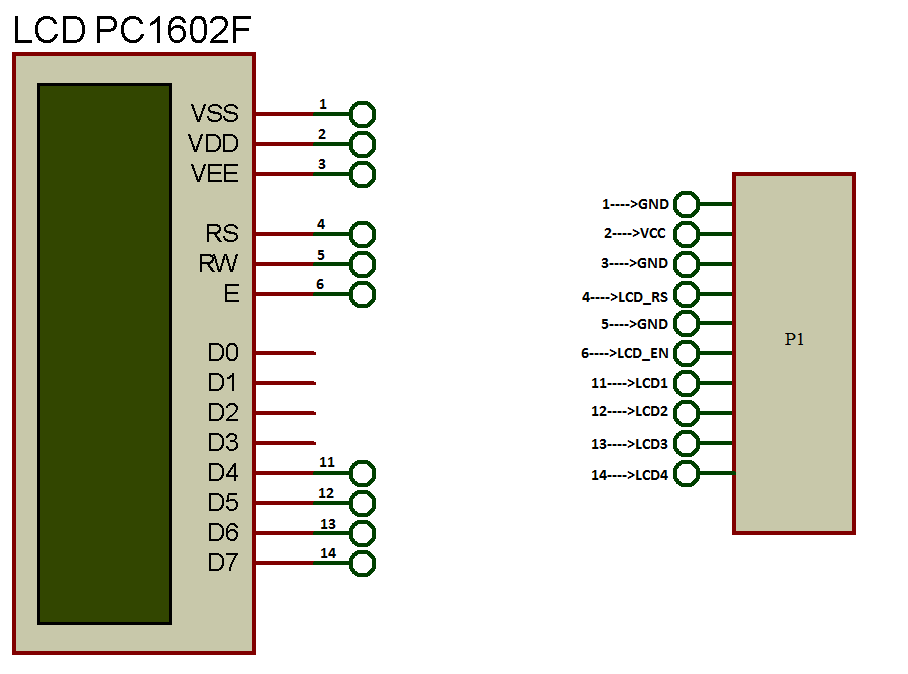
\includegraphics[width=12 cm]{figuras/lcd16x2.png}
\caption{Diagrama esquematico de conexion display LCD 16x2.}
\label{Fig31}
\end{figure}


\item[•]\textbf{Paso 4}: Ingresar sobre el archivo fuente creado en el paso 1, el código que contiene el archivo \textit{Ejemplo$\_$6.c}, ubicado sobre la carpeta \textit{EJ$\_$6$\_$BM}.
\item[•]\textbf{Paso 5}: Realizar la compilación y depuración del programa.
\end{enumerate}




\section{Sistema Operativo en Tiempo Real}
Un Sistema Operativo es un conjunto de programas que ayuda al programador de aplicaciones a gestionar recursos de hardware disponible, entre ellos el tiempo del procesador y la memoria.
Una parte del OS se encarga de asignar el tiempo de ejecución a todos los programas que tiene cargados en base a un juego de reglas conocido de antemano. A dichos subprogramas se los denomina Tareas.
Con esto se logra aparentar que múltiples programas se están ejecutando simultaneamente, sin embargo solo pueden hacerlo de uno a la vez.
El encargado de realizar esta gestión es un componente del sistema operativo denominado Scheduler o Programador de Tareas. La función de éste es determinar que tarea debe estar en ejecución a cada momento.
 \\
 
Ante la ocurrencia de ciertos eventos el Scheduler revisa si la tarea en ejecución debe reemplazarse por alguna otra tarea. A este reemplazo se lo denomina cambio de contexto de ejecución.
 \\
 
Debido a que el OS debe guardar el contexto completo de la tarea actual, y reemplazarlo por la tarea reentrante. Debe reservarse un bloque de la memoria de datos para cada tarea, lo cual limita el número de tareas que pueden ejecutarse de forma simultánea. Los cambios de contexto que se realizan cuando se reemplaza una tarea por otra no agregan trabajo al programador, de modo que al retornar a dicha tarea, el programador no observa ningún sintoma de haberla pausado alguna vez.
 \\
 
Un RTOS (sigla de \textit{Real Time Operating System}) realiza la misma función que un OS común, sin embargo agrega herramientas para que los programas de aplicación puedan cumplir compromisos temporales definidos por el programador. De modo que se encuentran diseñados para la administración de varias tareas simultáneas con plazos de tiempo estrictos.
 \\
 
El RTOS ofrece funcionalidad para asegurar que una vez ocurrido un evento, la respuesta ocurra en un tiempo acotado. Es necesario destacar que esto no lo hace por si solo sino que brinda al programador herramientas para implemetarlo de forma mas simple.

\subsection{Tareas}\label{sec:tareas}
El bloque básico de software escrito sobre un RTOS es la Tarea, sobre la mayoria de las RTOS que se ofrecen en el mercado, una Tarea es una simple subrutina.
 \\
 
Una Tarea provee un contexto en el cual se ejecuten las funciones, mientras que el Scheduler organiza la secuencia de ejecución de las tareas.
En algún punto del programa se produce el llamado a alguna función que produzca la ejecución de dicha tarea.
 \\
 
En el sistema operativo OSEK las Tareas deben ser definidas en la configuración, de manera que no es posible crear Tareas de forma dinámica (a diferencia de los Sistemas Operativos de escritorio). En el momento de la compilación se genera el código del sistema operativo y se definen la cantidad de Tareas y sus características. Además deben utilizarse macros para las definiciones y las funciones (a dichas funciones se las suele denominar Servicios del Sistema ) que ofrece este Sistema Operativo, para ello, debe incluirse sobre el programa, el archivo cabecera \textit{os.h}.
 \\
 
Este sistema operativo ofrece dos conceptos distintos de Tareas:
\begin{enumerate}
\item[•]Tareas del tipo \emph{BASIC}: Este tipo de Tareas solamente libera al procesador en los siguientes casos:
\begin{enumerate}
\item[•]Cuando terminan.
\item[•]Cuando son interrumpidas por acción del Scheduler, al realizar la activación de una Tarea que posea mayor prioridad (caracteristica propia de los Sistemas Operativos del tipo \textit{preemptive}).
\item[•]Ocurre una interrupción que causa que el procesador acuda a una subrutina de atencion de interrupción.
\end{enumerate}
\item[•]Tareas del tipo \emph{EXTENDED}: Se distinguen de las Tareas extendidas por el hecho de que pueden utilizar una funcion propia de este OS, denominado \textit{WaitEvent()}. Este tipo de Tareas permite liberar el procesador y ser relevado hacia Tareas de menor prioridad, sin la necesidad de que finalize la Tarea que se encuentra esperando.
%DECIDIR SI ESTO VA O NO..DADO QUE NO ENCUENTRO DE DONDE LO SAQUE%
La ventaja de las Tareas extendidas es que pueden manejar coherentemente una Tarea sin importar que eventos de sincronización se encuentren activos%%
\subsubsection{Modelo de Tareas Básicas}
El modelo de las Tareas Basicas es similar al de las Tareas Extendidas, excepto que éstas no contienen un estado \textit{Waiting}. A continuación se realiza una breve descripción de los estados definidos sobre este tipo de Tareas.
\begin{enumerate}
\item[•]\textbf{\emph{Running}}: En este estado, la CPU es asignada a la Tarea, de modo que se ejecutan sus instrucciones. Solamente una sola Tarea (sin importar de que tipo sea) puede estar en este estado, en un instante determinado; mientras las demás Tareas pueden adoptar otros estados.
\item[•]\textbf{\emph{Ready}}: Se cumplieron todos los pre-requisitos para que la Tarea adquiera el estado \textit{Running}.El \textit{Scheduler} decide cuál Tarea en estado \textit{Ready} será desplazada al estado \textit{Running}.
\item[•]\textbf{\emph{Suspended}}: En este estado, la Tarea se encuentra en estado pasivo y puede ser activada.
\end{enumerate}
La Figura \ref{Fig32} ilustra los conceptos explicados previamente.

\begin{figure}[H]
\centering
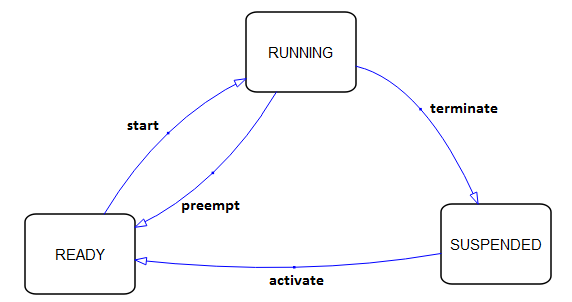
\includegraphics[width=10 cm]{figuras/f14.png}
\caption{Modelo de las Tareas del tipo \textit{BASIC}.}
\label{Fig32}
\end{figure}

\end{enumerate}

El Cuadro \ref{Tab3} explica los diferentes eventos que provocan las transiciones entre los estados. 

\begin{table}[h]

\resizebox{18cm}{!}{
\begin{tabular}{|l|l|l|l|}
\hline\hline
\textbf{{\Large Transicion}} & \textbf{{\Large Estado Actual}} & \textbf{{\Large Nuevo Estado}} & \textbf{{\Large Descripcion}}\\ \hline
\textbf{{\Large activate}}&{\Large suspended}&{\Large ready}&{\Large Una nueva tarea se asigna al estado} \textit{{\Large Ready}} {\Large por el OS}.\\ \hline
\textbf{{\Large start}}&{\Large ready}&{\Large running}&{\Large Una Tarea en estado} \textit{{\Large Ready}} {\Large es seleccionada por el} \textit{{\Large Scheduler}} {\Large para ser ejecutada}\\ \hline
\textbf{{\Large preempt}}&{\Large running}&{\Large ready}&{\Large El} \textit{{\Large Scheduler}} {\Large decide empezar otra Tarea. La Tarea que estaba en estado} \textit{{\Large Running}} {\Large se establece en estado} \textit{{\Large Ready}}.\\ \hline
\textbf{{\Large terminate}}&{\Large running}&{\Large suspended}&{\Large La tarea en estado} \textit{{\Large Running}} {\Large se establece en estado} \textit{{\Large Suspended}} {\Large gracias a la acción de algún servicio del sistema}.\\ \hline
\end{tabular}
}
\caption{Tabla de transiciones de las Tareas del tipo \textit{Basic}.}
\label{Tab3}

\end{table}

\subsubsection{Modelo de Tareas Extendidas}
El modelo de las Tareas Extendidas posee cuatro estados:
\begin{enumerate}
\item[•]\emph{\textbf{Running}}: En dicho estado, la CPU es asignada a la Tarea, de modo que se ejecuten las instrucciones que contiene la misma. Solamente una Tarea puede encontrarse en dicho estado en un instante determinado, mientras las otras Tareas pueden adoptar los demas estados.
\item[•]\emph{\textbf{Ready}}: Se cumplieron todos los pre-requisitos necesarios para la transición al estado \textit{Running}. El \textit{Scheduler} decide cuál de las tareas en estado \textit{Ready} será ejecutada a continuación.
\item[•]\emph{\textbf{Waiting}}: La ejecución de una Tarea no puede continuar debido a que debe $"$esperar$"$ a que un evento ocurra.
\item[•]\emph{\textbf{Suspended}}: La Tarea se encuentra en modo pasivo hasta que se active.
\end{enumerate}

La Figura \ref{Fig33} ilustra los conceptos explicados previamente.
\begin{center}
\begin{figure}[!h]
\centering
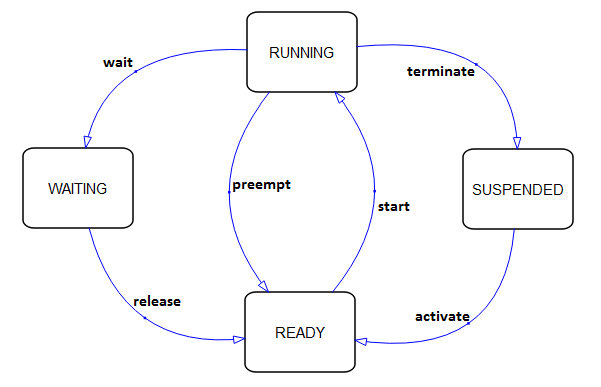
\includegraphics[width=10 cm]{figuras/f15.png}
\caption{Modelo de las Tareas del tipo \textit{EXTENDED}.}
\label{Fig33}
\end{figure}
\end{center}

El Cuadro \ref{Tab4} explica los diferentes eventos que provocan las transiciones entre los estados.
\begin{table}[H]

\resizebox{18cm}{!}{
\begin{tabular}{|l|l|l|l|}
\hline\hline
\textbf{{\LARGE Transicion}} & \textbf{{\LARGE Estado Actual}} & \textbf{{\LARGE Nuevo Estado}} & \textbf{{\LARGE Descripcion}}\\ \hline
\textbf{{\LARGE activate}}&{\LARGE suspended}&{\LARGE ready}&{\LARGE Una nueva tarea se asigna al estado }\textit{{\LARGE Ready}} {\LARGE por el OS}.\\ \hline
\textbf{{\Large start}}&{\Large ready}&{\Large running}&{\Large Una Tarea en estado} \textit{{\Large Ready}} {\LARGE es seleccionada por el} \textit{{\Large Scheduler}} {\Large para ser ejecutada}\\ \hline
\textbf{{\Large wait}}&{\Large running}&{\Large waiting}&{\Large La tarea se establece en estado} \textit{{\Large Waiting}} {\Large debido a la accion de un Servicio del Sistema.} \\ \hline
\textbf{{\Large release}}&{\Large waiting}&{\Large ready}&{\Large Al menos ocurrió un evento que esperaba la Tarea}\\ \hline
\textbf{{\Large preempt}}&{\Large running}&{\Large ready}&{\Large El} \textit{{\Large Scheduler}}{\Large decide iniciar otra Tarea. La Tarea que se encontraba en estado} \textit{{\Large Running}},{\Large  se establece en estado} \textit{{\Large Ready}}.\\ \hline
\textbf{{\Large terminate}}&{\Large runnning}&{\Large suspended}&{\Large La Tarea en estado} \textit{{\Large Running}} {\Large se establece al estado} \textit{{\Large Suspended}} {\Large gracias a un Servicio del Sistema}.
\end{tabular}
}
\caption{Transiciones de las Tareas del tipo \textit{Extended}.}
\label{Tab4}

\end{table}

\underline{Activación de Tareas}: 

La activación de una Tarea es realizada mediante el Servicio del Sistema \textit{ActivateTask} o por \textit{ChainTask}. Luego de la activación de una Tarea, ésta se encuentra lista para ejecutarse desde su primer instrucción. En el caso que se produzcan múltiples activaciones de una Tarea del tipo \textit{BASIC}, el Sistema Operativo OSEK almacena estas activaciones paralelas, siempre y cuando se haya definido sobre éste, una clase de conformidad.
 \\
 
\underline{Finalización de las tareas}:

En el Sistema Operativo OSEK, una Tarea solo puede finalizarse por acción propia, mediante el Servicio del Sistema \textit{TerminateTask}. Cabe destacar que el Servicio del Sistema \textit{ChainTask} provee una forma de realizar la activación de una Tarea determinada, justo después de la finalización de la Tarea que se encuentra corriendo.
 \\
 
Esta estrictamente prohibido realizar una Tarea que no finalize con alguno de estos dos Servicios del Sistema, dado que puede ocasionar un comportamiento indefinido.
 \\
 
\underline{Prioridad de las tareas}:

La asignación de prioridades sobre las Tareas se realiza a través de la definición de números enteros desde 0 hasta 255. Mientras mayor es el valor del numero, mayor será la prioridad.Una Tarea que se encuentra corriendo, no puede ser interrumpida por una de menor o igual prioridad.
\subsection{Scheduler}\label{sec:scheduler}
El algoritmo del Scheduler puede ser visto fundamentalmente como un coordinador de Tareas con las prioridades ya establecidas, en el cual se define un número máximo de activaciones de las mismas. El sistema operativo OSEK define tres politicas de \textit{Scheduling}, las cuales se mencionan a continuación.
 \\
 
\underline{\textit{Scheduling Full Preemptive}}:

Esta politica de \textit{Scheduling} implica que una Tarea que se encuentra en el estado \textit{Running} puede ser interrupida sobre cualquier instrucción, como consecuencia de la ocurrencia de alguna condición o evento; que ya se encuentre definido previamente sobre el OS. \textit{Full Preemptive Scheduling} determinará que una Tarea en el estado \textit{Running} sea establecido en el estado \textit{Ready}, tan pronto como una Tarea de mayor prioridad se establezca en estado \textit{\textit{Ready}}.
 \\
 
El contexto de la Tarea será almacenado de forma que la Tarea que fue interrumpida pueda continuar sobre la instancia en donde fue interrumpida.
 \\
 
\underline{\textit{Scheduling Non Preemptive}}:

Cuando el cambio de Tareas solo se produce mediante la ejecución de algún Servicio del Sistema (explicitados en los puntos de \textit{Scheduling}).
 \\
 
\underline{Puntos de \textit{Scheduling}}:

\begin{enumerate}
\item[•]Puntos de \textit{Scheduling} en una tarea \textit{NON-PREEMPTIVE}
\begin{enumerate}
\item[•]Al llamar a la interfase \textit{Schedule} cuando retorna E$\_$OK.
\end{enumerate}
\item[•]Puntos de \textit{Scheduling} en una tarea \textit{PREEMPTIVE}
\begin{enumerate}
\item[•]Al finalizar un llamado a la interfase \textit{ActivateTask} que retorna E$\_$OK.
\item[•]Al finalizar un llamado a la interfase \textit{ChainTask} que no retorna.
\item[•]Al finalizar un llamado a la interfase \textit{TerminateTask} que no retorna.
\item[•]Al finalizar un llamado a la interfase \textit{ReleaseResource} que retorna E$\_$OK.
\item[•]Al finalizar un llamado a la interfase \textit{SetEvent} que no retorna.
\item[•]Al expirar una alarma que activa una tarea.
\item[•]Al terminar la ejecución de una ISR de categoría 2
\end{enumerate}
\end{enumerate} 

\subsection{Modos de Aplicación}
Los Modos de Aplicación son designados sobre un Sistema Operativo OSEK, para trabajar sobre diferentes modos de operación. El número mínimo de modos de aplicación que puede soportar este Sistema Operativo es igual a 1. Un ejemplo que puede ilustrarse es la definición de dos modos de operación, uno para la operación normal del programa, y otro para la finalización de la misma.

\subsection{Eventos}

Los eventos son objetos manejados por el OS. Es posible considerarla de forma abstracta como un bit o un flag, que puede ser enmascarado. Dichos eventos pueden ser seteados o restablecidos utilizando Servicios del Sistema. Es importante destacar que solamente las Tareas del tipo \textit{EXTENDED} pueden utilizar esta herramienta para permitir la sincronización de las mismas. El Servicio del Sistema \textit{WaitEvent} permite esperar al suceso del evento, para poder realizar las instrucciones que contenga dicha Tarea.
 \\
 
Las Tareas del tipo \textit{EXTENDED} típicamente poseen su propio \textit{stack} o pila que registra el suceso de dicho evento. Sin embargo, es muy importante destacar que este tipo de Tareas solo pueden ser activadas una sola vez.
 \\
 
Un evento individual es identificado por el propietario de dicho evento, y por su nombre (denominado Máscara según la especificación). Cuando una Tarea de tipo \textit{EXTENDED} es activada, los eventos asignados a la misma son establecidos a 0 por el OS. El significado de un evento es definido por la aplicación; por ejempo, puede significar que ha expirado un \textit{Timer}, puede significar que se encuentra disponible un recurso, puede significar la recepción de un mensaje, etc.
 \\
 
Existen varias opciones disponibles para manipular los eventos, tanto para las Tareas que son propietarias de dicho Evento, como de las demás Tareas que no son propietarias del Evento, las cuales no necesariamente deben ser Tareas del tipo \textit{EXTENDED}.
 \\
 
Todas las Tareas e Interrupciones del tipo \textit{ISR2} pueden indicar el suceso de un Evento e informarlo a la Tarea propietaria del evento (del tipo \textit{EXTENDED}) siempre y cuando no se encuentre en estado \textit{SUSPENDED}. Sin embargo, solamente la Tarea propietaria de dicho Evento puede restablecer el flag del Evento.
 \\
 
Debe destacarse que cuando una Tarea tipo \textit{EXTENDED}, se encuentra en estado \textit{Waiting}, se establece en el estado \textit{Ready} si al menos ocurre uno de los Eventos que dicha Tarea estaba esperando. Si una Tarea tipo \textit{EXTENDED} se encuentra ejecutándose y trata de esperar un Evento que ya haya ocurrido, dicha Tarea se mantiene en el estado \textit{Running}.

\subsection{Clases de Conformidad}
Con la finalidad de permitir que OSEK-OS pueda ser utilizado en una gran variedad de sistemas con diferentes capacidades y demandas (por ejemplo memoria, capacidad de procesamiento, etc.) es que OSEK-OS define 4 clases de conformidad (CC).
 \\
 
Las diferentes clases existen para poder comparar entre sistemas, agrupar las interfaces según la clase de conformidad y facilitar la certificación de conformidad. Las clases de conformidad se determinan según los siguientes atributos: 

\begin{enumerate}
\item[•]Múltiple activaciónde tareas básicas.
\item[•]Tipos de tareas aceptadas: básicas y extendidas.
\item[•]Cantidad de tareas por prioridad.
\end{enumerate}

De esta forma se definen las siguientes clases de conformidad:
\begin{enumerate}
\item[•]BCC1: que soporta únicamente tareas  básicas con máximo una activación por tarea, y todas las tareas con prioridad diferente.
\item[•]BCC2: como  BCC1 pero con más de una tarea por prioridad y las tareas soportan más de una activación.
\item[•]ECC1: como BCC1 pero con tareas extendidas.
\item[•]ECC2: como  ECC1 pero con más de una tarea por prioridad y las tareas soportan más de una activación.
\end{enumerate}
El OSEK-OS de la CIAA soporta todas las conformidades. Dependiendo de esta configuración el sistema decidirá si se implementa una clase BCC1 o ECC2. Por lo que para el usuario final del CIAA-Firmware es prácticamente irrelevante conocer las clases. El Firmware decide automáticamente y configura la clase de conformidad correcta según los requerimientos del usuario.La Figura \ref{Fig34} ilustra los conceptos presentados anteriormente.


\begin{figure}[H]
\centering
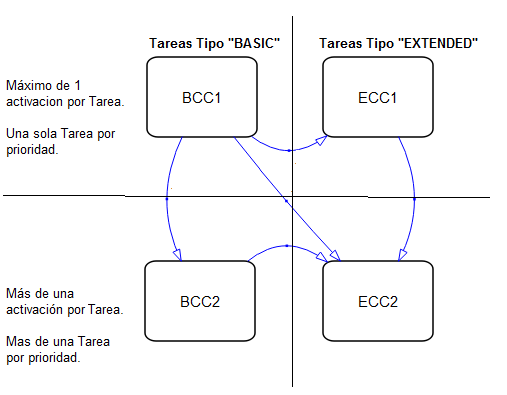
\includegraphics[width=8 cm]{figuras/f17.png}
\caption{Clases de Conformidad.}
\label{Fig34}
\end{figure}

\subsection{Configuración y Generación}\label{sec:generacionoil}
Al ser OSEK-OS un sistema estático es necesario configurarlo: La cantidad de tareas, que prioridad tienen las mismas, el tamaño de pila que utilizan, etc.
  \\
  
Para ello OSEK-VDX definió otro estándar llamado OSEK Implementation Language comúnmente llamado OIL.
 \\
 
OIL es un lenguaje textual con una sintaxis similar al lenguaje C donde se indican las características del sistema operativo como ser: tareas, prioridades, pila, interrupciones etc. El siguiente ejemplo ilustra al usuario sobre la generación de dicho archivo.
 \\
 
Es necesario destacar que para la utilización de \textit{RTOS OSEK} utilizando instrucciones en \textit{LPCOpen versión 2.17}, se debe eliminar la definiciones de \textit{TRUE/FALSE} del tipo \textit{boolean} que realiza \textit{LPCOpen} de forma que no genere conflictos con las definiciones propias del Sistema Operativo. La Figura \ref{errorboolean} ilustra una ventana resultante del error en el caso que no se haya realizado la eliminacion de dicha definicion.

\begin{figure}[!h]
\centering
\includegraphics[width=18 cm]{figuras/f24.png}
\caption{Mensaje de consola de error por conflicto de definiciones de valores lógicos.}
\label{errorboolean}
\end{figure}
Para solventar dicho error, una alternativa propuesta es la siguiente:
\begin{enumerate}
\item[•]Sobre el \textit{Firmware} del proyecto, el usuario debe dirigirse hacia:

\textit{Firmware/externals/drivers/cortexM4/lpc43xx/inc/lpc$\_$types.h}.
\item[•]Comentar la instrucción \textit{typedef enum {FALSE =0, TRUE=!FALSE} Bool}. La Figura \ref{eliminacion} ilustra dicha instrucción comentada:
\begin{figure}[!h]
\centering
\includegraphics[width=12 cm]{figuras/f25.png}
\caption{Eliminación de definición de variables lógicas en \textit{LPCOpen}.}
\label{eliminacion}
\end{figure}
\end{enumerate}\underline{Archivos Makefile utilizados sobre cada ejemplo}: \\
Otro aspecto que es necesario destacar es que para la implementación de los siguientes ejemplos se utiliza el archivo \textit{Makefile} proporcionado en los ejemplos del \textit{Firmware} de la \textit{CIAA}.
\subsection{Implementación de ejemplo N$^{\circ}$1: Tareas en OSEK}\label{sec:tareasOSEK}
Este ejemplo utiliza los leds de la placa y un Display 7 Segmentos, para implementar un contador de numeros decimales, a través de una sola Tarea del tipo \textit{BASIC}.
\begin{enumerate}

\item[•]\textbf{Paso 1}: En primer lugar es necesario generar el archivo OIL para configurar el Sistema Operativo OSEK. A través del \textit{Bloc de Notas} o a través de cualquier editor de texto, debe almacenarse el archivo de configuracion de tipo \textit{OIL} sobre la carpeta \textit{etc} previamente creada sobre el directorio del proyecto, en dicho archivo, debe iniciar la configuración a través de la sintaxis \textit{OSEK OSEK} y sobre los simbolos ``$\lbrace$'' y ``$\rbrace$'' ,se determinarán los restantes aspectos que tendra el OS. La Figura \ref{Fig35} ilustra lo mencionado anteriormente.
\begin{figure}[H]
\centering
\includegraphics[width=5 cm]{figuras/f18.png}
\caption{Inicio de Archivo de Configuración.}
\label{Fig35}
\end{figure}
\item[•]\textbf{Paso 2}: Luego debe definirse mediante la sintaxis \textit{OS}, el nombre del sistema operativo (el cual es arbitrario, dado que se ha especificado en la instruccion anterior que se implementa un sistema operativo OSEK), la Figura \ref{Fig36} ilustra el concepto explicado anteriormente.
\begin{figure}[H]
\centering
\includegraphics[width=5 cm]{figuras/f19.png}
\caption{Archivo de Configuración. Comienzo de especificación.}
\label{Fig36}
\end{figure}

\item[•]\textbf{Paso 3}: A continuación debe definirse las siguientes configuraciones para el OS del ejemplo:
\begin{enumerate}
\item[•]\textbf{Paso 3.1}: El nivel de chequeo de errores que se pueden producir. Existen dos niveles que pueden determinarse: 
\begin{enumerate}
\item[•]\textit{STANDARD}: Implica un chequeo mínimo de errores, se encuentra pensado para el empleo en sistemas que deben producirse en masa.La instrucción utilizada es \textit{OS = STANDARD}. 
\item[•]\textit{EXTENDED}: Implica un chequeo máximo de errores y \textit{debug hooks}. La instrucción utilizada es \textit{OS = EXTENDED}.
\end{enumerate}
\item[•]\textbf{Paso 3.2}: Funciones implementadas por el usuario que el OS llamará en circunstancias específicas, tales como:
\begin{enumerate}
\item[•]\textit{Startuphook}: Es  llamada  durante  la  inicialización  del  sistema  operativo,  antes  de  ser completada. En caso de utilizarla se debe escribir la instrucción \textit{STARTUPHOOK = TRUE}; en caso contrario se debe asignar \textit{FALSE}.
\item[•]\textit{Shutdownhook}: Es llamada al finalizar el apagado del sistema operativo. En caso de utilizarla se debe escribir la instrucción \textit{SHUTDOWNHOOK = TRUE}; en caso contrario se debe asignar \textit{FALSE}.
\item[•]\textit{Pretaskhook}: Es llamada antes de proceder a ejecutar una tarea. En caso de utilizarla se debe escribir la instrucción \textit{PRETASKHOOK = TRUE}; en caso contrario se debe asignar \textit{FALSE}.
\item[•]\textit{Posttaskhook}: Es llamada al finalizar la ejecución de una tarea. En caso de utilizarla se debe escribir la instrucción \textit{POSTTASKHOOK = TRUE}; en caso contrario se debe asignar \textit{FALSE}.
\item[•]\textit{Errorhook}: Es llamada en caso de que alguna de las interfaces del sistema operativo retorne un valor distinto a E$\_$OK. En caso de utilizarla se debe escribir la instrucción \textit{ERRORHOOK = TRUE}; en caso contrario se debe asignar \textit{FALSE}.
\end{enumerate}
\item[•]\textbf{Paso 3.3}: Uso del \textit{Scheduler} como recurso mediante el atributo \textit{USERESSCHEDULER}.
\item[•]\textbf{Paso 3.4}: Uso del mapa de memoria mediante el atributo \textit{MEMMAP}.
\end{enumerate}
 
La Figura \ref{Fig37} ilustra un OS configurado de forma que el nivel de chequeo de errores sea el mínimo, no se determine el uso del \textit{Scheduler}, y no se utilize una cantidad específica de memoria, por último solamente se define una función en caso de un error producido en el OS.
\begin{figure}[H]
\centering
\includegraphics[width=8 cm]{figuras/f20.png}
\caption{Ejemplo de especificación de OS sobre archivo OIL.}
\label{Fig37}
\end{figure}

\item[•]\textbf{Paso 4}: Luego de la configuración inicial del Sistema Operativo debe determinarse una variable denominada "Modo de aplicación", ésta define diferentes modos de operación para la aplicación. No existen atributos estándares definidos para esta variable, por lo que comúnmente se lo define en el archivo de configuración OIL como \textit{APPMODE=AppMode1}.
\begin{enumerate}
\item[•]\textbf{Paso 4.1}: Declarar el recurso utilizado por el módulo \textit{POSIX} del Firmware de la CIAA, mediante la sintaxis \textit{POSIXR}.
\item[•]\textbf{Paso 4.2}: Declarar el evento utilizado por el módulo \textit{POSIX} del Firmware de la CIAA, mediante la sintaxis \textit{POSIXE}.
La Figura \ref{paso42} ilustra las declaraciónes realizadas:
\begin{figure}[H]
\centering
\includegraphics[width=4 cm]{figuras/f48.png}
\caption{Definición de APPMODE, Recurso POSIXE, Recurso POSIXR.}
\label{paso42}
\end{figure}
\end{enumerate}

\item[•]\textbf{Paso 5}: A continuación se define una Tarea que efectua la configuración inicial de la placa, y de los puertos GPIO utilizados para el Display 7 Segmentos. La instrucción que permite la definición de una Tarea sobre el archivo de configuracion \textit{OIL} es \textit{TASK}, la Figura \ref{Fig38} ilustra el proceso llevado a cabo.
\begin{figure}[H]
\centering
\includegraphics[width=15 cm]{figuras/f21.png}
\caption{Definición de Tarea sobre archivo de configuración.}
\label{Fig38}
\end{figure}
Debe destacarse que la implementación de OSEK que se utiliza en este caso, nos permite realizar la asignación de memoria de programa para una Tarea a través del atributo \textit{TASK}, el valor asignado es un número entero que representa la cantidad de memoria en Bytes. Si se define una cantidad de memoria demasiado chica, es posible generar un error grave en el código dado que el contador de programa puede direccionarse sobre zonas de la memoria que no fueron designadas para la Tarea creada, dicho problema se lo denomina \textit{stack overflow}.

\item[•]\textbf{Paso 6}: La tarea que se desea definir en primer lugar, necesita activarse en el momento de inicio del programa. Teniendo en cuenta los atributos explicados sobre la Figura \ref{Fig38} ,se determina que \textit{AUTOSTART} adquiera el valor \textit{TRUE}. Dado que no se prevee que dicha Tarea vuelva a ejecutarse durante el desarrollo del programa, se asigna una prioridad baja y su tipo designado es \textit{BASIC}. La Figura \ref{inicializar} ilustra la definición de dicha Tarea.
\begin{figure}[H]
\centering
\includegraphics[width=4 cm]{figuras/f47.png}
\caption{Definición de Tarea INICIALIZAR sobre Ejemplo N$^{\circ}$1.}
\label{inicializar}
\end{figure}
\item[•]\textbf{Paso 7}: La siguiente Tarea realiza la muestra de los digitos sobre los leds incorporados en la placa (forma binaria) y sobre el Display 7 Segmentos. Es importante destacar que esta Tarea se ejecuta constantemente, debido a que no existe otra Tarea de mayor prioridad que se active e interrumpa su ejecución. Para permitir esta ejecución constante es necesario la instrucción propia del SO (también denominada Servicio del Sistema) \textit{ChainTask()} para permitir que esta Tarea se reactive a si misma. La Figura \ref{Fig39} ilustra las definiciones de las dos Tareas descriptas anteriormente.
\begin{figure}[H]
\centering
\includegraphics[width=8 cm]{figuras/f22.png}
\caption{Ilustración de definición de Tareas de Ejemplo N$^{\circ}$1.}
\label{Fig39}
\end{figure}
\item[•]\textbf{Paso 8}: A continuación debe crearse el directorio que contiene el proyecto a implementar, para ello, es posible seguir los Pasos 1, 2 y 3 de la Seccion \ref{sec:ej1sapi}. Es necesario destacar la necesidad de crear un directorio adicional sobre el proyecto, cuyo nombre debe ser \textit{etc}. Sobre dicho directorio debe almacenarse el archivo de configuración OIL. 
\item[•]\textbf{Paso 9}: Debido a que no todos los módulos que integra la librería \textit{sAPI} son compatibles con el Sistema Operativo, debemos especificar sobre el proyecto cuáles son los módulos a utilizar. En primer lugar debemos copiar y pegar aquellos archivos cabeceras de los módulos (compatibles) sobre la carpeta \textit{inc} y sus correspondientes archivos fuentes sobre la carpeta \textit{src}. A continuación se detalla una lista (respecto la version 0.3.0) de éstos modulos:
\begin{enumerate}
\item[•]\textit{sAPI$\_$AnalogIO.h}
\item[•]\textit{sAPI$\_$Board.h}
\item[•]\textit{sAPI$\_$DataTypes.h}
\item[•]\textit{sAPI$\_$DigitalIO.h}
\item[•]\textit{sAPI$\_$Hmc5883l.h}
\item[•]\textit{sAPI$\_$I2c.h}
\item[•]\textit{sAPI$\_$PeripheralMap.h}
\item[•]\textit{sAPI$\_$Rtc.h}
\item[•]\textit{sAPI.h}
\end{enumerate}
En particular el módulo \textit{sAPI$\_$Uart} puede ser compatible en el caso que se borren los Handler de interrupción. Para ello, el usuario puede comentar la sección del código (ilustrado sobre la Figura \ref{modificacionuart}) sobre \textit{sAPI$\_$Uart.h}.
\begin{figure}[H]
\centering
\includegraphics[width=10 cm]{figuras/f29.png}
\caption{Modificación para compatibilidad de módulo sAPI$\_$Uart. Parte 1.}
\label{modificacionuart}
\end{figure}

Sobre el archivo \textit{sAPI$\_$Uart.c}, debe realizar las modificaciones que se muestran en las Figuras \ref{modificacionuart2} y \ref{modificacionuart3}.
\begin{figure}[H]
\centering
\includegraphics[width=8 cm]{figuras/f30.png}
\caption{Modificación para compatibilidad de módulo sAPI$\_$Uart. Parte 2.}
\label{modificacionuart2}
\end{figure}
\begin{figure}[H]
\centering
\includegraphics[width=10 cm]{figuras/f31.png}
\caption{Modificación para compatibilidad de módulo sAPI$\_$Uart. Parte 3.}
\label{modificacionuart3}
\end{figure}

\item[•]\textbf{Paso 10}: Para finalizar la inclusión de dichos módulos, el usuario debe eliminar las inclusiones realizadas sobre el archivo cabecera \textit{sAPI.h}. La Figura \ref{ejemploinclusion} ejemplifica la inclusión de el módulo \textit{sAPI$\_$DigitalIO.h}.

\begin{figure}[H]
\centering
\includegraphics[width=7 cm]{figuras/f32.png}
\caption{Ejemplo de inclusion de módulo de entradas y salidas digitales.}
\label{ejemploinclusion}
\end{figure}
Debe destacarse que es necesaria la inclusión de las librerias \textit{sAPI$\_$Board.h},\textit{sAPI$\_$DataTypes.h} y \textit{sAPI$\_$PeripheralMap.h}. En primer lugar para la definición de la placa a utilizar, en segundo lugar los tipos de datos definidos por la librería, y por último para la inclusión de las definiciónes de los terminales para los periféricos.\\
\item[•]\textbf{Paso 11}: Realizar la inclusión de las bibliotecas \textit{dsp7seg} y \textit{digitos}, de la misma forma que se realiza sobre el paso 9.
\item[•]\textbf{Paso 12}: Sobre el archivo fuente del proyecto, ingresar el código proporcionado en el tutorial.

\end{enumerate}
%\underline{Generación de archivo OIL}:

\subsection{Implementación de ejemplo N$^{\circ}$2: Múltiples Tareas en OSEK}

El siguiente ejemplo pretende demostrar como pueden implementarse varias Tareas del Tipo \textit{BASIC} a través de las instrucciónes del Sistema Operativo \textit{TerminateTask()} y \textit{ChainTask()}.

En este caso, se desea implementar un programa que  permita encender los leds incorporados en la placa de izquierda a derecha, oprimiendo \textit{TEC1, TEC2, TEC3, TEC4} en el mismo orden.
\begin{enumerate}
\item[•]\textbf{Paso 1}: Realizar la creación del archivo de configuración OIL siguiendo los pasos 1, 2 y 3 de la Sección \ref{sec:tareasOSEK}.
\item[•]\textbf{Paso 2}: Definir los Eventos, Recursos y Modo de Aplicación que se determina sobre el paso 5 de la Sección \ref{sec:tareasOSEK}.
\item[•]\textbf{Paso 3}: Definir el recurso \textit{tecla$\_$recurso} de forma similar a la que se realiza sobre el paso anterior. Este recurso se define por propósito ilustrativo, dado que se pretende mostrar como puede asignarse un recurso para una Tarea.
\item[•]\textbf{Paso 4}: Realizar la creación de la Tarea INICIALIZAR, cuyos atributos y variables asignadas son las mismas que las implementadas sobre el Ejemplo N$^{\circ}$1.
\item[•]\textbf{Paso 5}: Realizar la creación de la Tarea LEDRGB, que presenta las siguientes características:
\begin{enumerate}
\item[•]Prioridad: 5
\item[•]Número máximo de activaciones múltiples: 1
\item[•]Asignación de memoria de programa: 256 Bytes.
\item[•]Tipo de Tarea: BASIC
\item[•]Sin interrupciones por activación de otra Tarea de mayor prioridad.
\item[•]Recurso: POSIXR
\end{enumerate}
\item[•]\textbf{Paso 6}: Realizar la creación de la Tarea LEDUNO, que presenta las siguientes características:
\begin{enumerate}
\item[•]Prioridad: 4
\item[•]Número máximo de activaciones múltiples: 1
\item[•]Asignación de memoria de programa: 256 Bytes.
\item[•]Tipo de Tarea: BASIC
\item[•]Sin interrupciones por activación de otra Tarea de mayor prioridad.
\item[•]Recurso: tecla$\_$recurso
\end{enumerate}
\item[•]\textbf{Paso 7}: Realizar la creación de la Tarea LEDDOS, que presenta las siguientes características:
\begin{enumerate}
\item[•]Prioridad: 3
\item[•]Número máximo de activaciones múltiples: 1
\item[•]Asignación de memoria de programa: 256 Bytes.
\item[•]Tipo de Tarea: BASIC
\item[•]Sin interrupciones por activación de otra Tarea de mayor prioridad.
\item[•]Recurso: tecla$\_$recurso
\end{enumerate}
\item[•]\textbf{Paso 8}: Realizar la creación de la Tarea LEDTRES, que presenta las siguientes características:
\begin{enumerate}
\item[•]Prioridad: 3
\item[•]Número máximo de activaciones múltiples: 1
\item[•]Asignación de memoria de programa: 256 Bytes.
\item[•]Tipo de Tarea: BASIC
\item[•]Sin interrupciones por activación de otra Tarea de mayor prioridad.
\item[•]Recurso: tecla$\_$recurso
\end{enumerate}
\item[•]\textbf{Paso 9}: Realizar la creación del directorio tal como se establece sobre el paso 8 en la Sección \ref{sec:tareasOSEK}.
\item[•]\textbf{Paso 10}: Incluir los módulos compatibles de la \textit{sAPI}, como se establece sobre los pasos 9 y 10 en la Sección \ref{sec:tareasOSEK}.
\item[•]\textbf{Paso 11}: Sobre el archivo fuente del proyecto, ingresar el código proporcionado por el tutorial.
\end{enumerate}

\subsection{Implementación de ejemplo N$^{\circ}$3: Eventos en OSEK}
Este ejemplo pretende brindar al usuario una introducción al manejo de las Tareas del tipo \textit{EXTENDED} a través de los Eventos. Se desea encender el \textit{LED1} de la placa al presionar la tecla \textit{TEC1}, y posteriormente encender el \textit{LED2} al presionar la tecla \textit{TEC2}.
 \\
 
Para ello se definen dos Tareas, una de ellas se denomina \textit{LED$\_$1} y la otra \textit{LED$\_$2}. Cuando inicia el Sistema Operativo, luego de la configuración inicial (llevada a cabo por una Tarea denominada INICIALIZAR), se ingresa a la Tarea \textit{LED$\_$1}, sobre la cual se implementa una estructura condicional \textit{while}, en la cual el código ingresa cuando la tecla \textit{TEC1} no ha sido oprimida; dentro de dicha estructura lógica se realiza la reactivación de la Tarea \textit{LED$\_$1}.
 \\
 
Sin embargo, al apretar la tecla correspondiente, se realiza el encendido de \textit{LED1} y posteriormente se ejecuta la activación de la Tarea \textit{LED$\_$2}, luego se realiza el establecimiento de el Evento \textit{tecla$\_$1}. Esto provoca que se ejecuten las instrucciones llevadas a cabo en la Tarea \textit{LED$\_$2}, dichas instrucciones realizan una acción similar. Sobre la Figura \ref{ejemplo3} se ilustra el concepto anterior:

\begin{figure}[H]
\centering
\includegraphics[width=10 cm]{figuras/f26.png}
\caption{Transición de las Tareas mediante Eventos en Ejemplo N$^{\circ}$3.}
\label{ejemplo3}
\end{figure}

\begin{enumerate}
\item[•]\textbf{Paso 1}: Realizar la creación del archivo de configuración OIL siguiendo los pasos 1, 2 y 3 de la Sección \ref{sec:tareasOSEK}.
\item[•]\textbf{Paso 2}: Definir los Eventos, Recursos y Modo de Aplicación que se determina sobre el paso 5 de la Sección \ref{sec:tareasOSEK}.
\item[•]\textbf{Paso 3}: Definir el recurso \textit{tecla$\_$recurso} de forma similar a la que se realiza sobre el paso anterior. Este recurso se define por propósito ilustrativo, dado que se pretende mostrar como puede asignarse un recurso para una Tarea.
\item[•]\textbf{Paso 4}: Definir los eventos \textit{tecla1} y \textit{tecla2}
\item[•]\textbf{Paso 5}: Realizar la creación de la Tarea INICIALIZAR, cuyos atributos y variables asignadas son las mismas que las implementadas sobre el Ejemplo N$^{\circ}$1.

\item[•]\textbf{Paso 6}: Realizar la creación de la Tarea LED$\_$1, que presenta las siguientes características:
\begin{enumerate}
\item[•]Prioridad: 3
\item[•]Número máximo de activaciones múltiples: 1
\item[•]Asignación de memoria de programa: 512 Bytes.
\item[•]Tipo de Tarea: EXTENDED
\item[•]Sin interrupciones por activación de otra Tarea de mayor prioridad.
\item[•]Recurso: tecla$\_$recurso
\item[•]Evento: tecla1
\end{enumerate}

\item[•]\textbf{Paso 7}: Realizar la creación de la Tarea LED$\_$2, que presenta las siguientes características:
\begin{enumerate}
\item[•]Prioridad: 3
\item[•]Número máximo de activaciones múltiples: 1
\item[•]Asignación de memoria de programa: 512 Bytes.
\item[•]Tipo de Tarea: EXTENDED
\item[•]Sin interrupciones por activación de otra Tarea de mayor prioridad.
\item[•]Recurso: tecla$\_$recurso
\item[•]Evento: tecla2
\end{enumerate}
\item[•]\textbf{Paso 8}: Realizar la creación del directorio tal como se establece sobre el paso 8 en la Sección \ref{sec:tareasOSEK}.
\item[•]\textbf{Paso 9}: Incluir los módulos compatibles de la \textit{sAPI}, como se establece sobre los pasos 9 y 10 en la Sección \ref{sec:tareasOSEK}.
\item[•]\textbf{Paso 10}: Sobre el archivo fuente del proyecto, ingresar el código proporcionado por el tutorial.

\end{enumerate}

\subsection{Alarmas}
Las alarmas son herramientas que proporciona el Sistema Operativo \textit{OSEK} para la ejecución de una acción luego de determinado tiempo.Éstas pueden realizar tres tipos de acciones:
\begin{enumerate}
\item[•]Activar una tarea.
\item[•]Establecer un evento de una tarea.
\item[•]Llamar una callback (retrollamada) en C.
\end{enumerate}
Para la implementación de las alarmas, ya sean que se utiliza una ó más alarmas el sistema operativo necesita un contador de hardware. Con un contador es posible configurar la cantidad de alarmas que sean necesarias.

Luego de que dicha alarma expire, solo puede realizar una sola acción, la cual es definida en el archivo de configuracion \textit{OIL} a traves de la variable \textit{ACTION}. A continuación se detalla los posibles parametros que pueden ingresarse:
\begin{enumerate}
\item[•]\textit{ACTIVATETASK} define la activación de una Tarea cuando dicha alarma expire.
\item[•]\textit{SETEVENT} Permite establecer un Evento (perteneciente a una Tarea) cuando dicha alarma expire.
\item[•]\textit{ALARMCALLBACK} define el nombre de la rutina \textit{callback} cuando la alarma expira.
\end{enumerate}
\subsection{Implementación de ejemplo N$^{\circ}$4: Eventos y Alarmas en OSEK}
Este ejemplo permite introducir al usuario en la utilización de alarmas para la temporización de acciones. Se pretende elaborar dos secuencias de luces a traves de los leds instalados en la placa, la primera de ellas se activa al oprimir la tecla \textit{TEC1}, mientras que la segunda se activa al oprimir \textit{TEC2}.

Sobre el archivo de configuración se definen dos Tareas en particular: \textit{SECUENCIA1} y \textit{SECUENCIA2}. Dichas Tareas se activan y ejecutan sus correspondientes códigos a través del establecimiento del Evento \textit{primersecuencia} o \textit{segsecuencia}.

Durante la ejecución de las Tareas \textit{SECUENCIA1} o \textit{SECUENCIA2} se identifica el Evento ocurrido, a través de las instrucciones \textit{WaitEvent()}y \textit{GetEvent()}. Definiendo como tipo de variable para la máscara de los Eventos de las Tareas, como \textit{Eventos1} y \textit{Eventos2} respectivamente.

En caso de que haya ocurrido el Evento \textit{primersecuencia} o \textit{segsecuencia}, los códigos de las Tareas proceden a activar las Alarmas \textit{Set$\_$Event$\_$tiempo1} y \textit{Set$\_$Event$\_$tiempo2} respectivamente, para lograr la temporización deseada en las secuencias.

\begin{enumerate}
\item[•]\textbf{Paso 1}: Realizar la creación del archivo de configuración OIL siguiendo los pasos 1, 2 y 3 de la Sección \ref{sec:tareasOSEK}.
\item[•]\textbf{Paso 2}: Definir los Eventos, Recursos y Modo de Aplicación que se determina sobre el paso 5 de la Sección \ref{sec:tareasOSEK}.
\item[•]\textbf{Paso 3}: Definir el recurso \textit{secuencia$\_$res} de forma similar a la que se realiza sobre el paso anterior. Este recurso se define por propósito ilustrativo, dado que se pretende mostrar como puede asignarse un recurso para una Tarea.
\item[•]\textbf{Paso 4}: Definir los eventos \textit{primersecuencia}, \textit{segsecuencia}, \textit{tiempo1} y \textit{tiempo2}.
\item[•]\textbf{Paso 5}: Realizar la creación de la Tarea INICIALIZAR, cuyos atributos y variables asignadas son las mismas que las implementadas sobre el Ejemplo N$^{\circ}$1.
\item[•]\textbf{Paso 6}: Realizar la creación de la Tarea TECLA, que presenta las siguientes características:
\begin{enumerate}
\item[•]Prioridad: 10
\item[•]Número máximo de activaciones múltiples: 1
\item[•]Asignación de memoria de programa: 256 Bytes.
\item[•]Tipo de Tarea: BASIC
\item[•]Sin interrupciones por activación de otra Tarea de mayor prioridad.
\item[•]Recurso: POSIXR
\end{enumerate}
\item[•]\textbf{Paso 7}: Realizar la creación de la Tarea SECUENCIA1, que presenta las siguientes características:
\begin{enumerate}
\item[•]Prioridad: 9.
\item[•]Número máximo de activaciones múltiples: 1.
\item[•]Asignación de memoria de programa: 256 Bytes.
\item[•]Tipo de Tarea: EXTENDED.
\item[•]Con interrupciones por activación de otra Tarea de mayor prioridad.
\item[•]Recurso: secuencia$\_$res.
\item[•]Evento: primersecuencia.
\end{enumerate}
\item[•]\textbf{Paso 8}: Realizar la creación de la Tarea SECUENCIA2, que presenta las siguientes características:
\begin{enumerate}
\item[•]Prioridad: 9.
\item[•]Número máximo de activaciones múltiples: 1.
\item[•]Asignación de memoria de programa: 256 Bytes.
\item[•]Tipo de Tarea: EXTENDED.
\item[•]Con interrupciones por activación de otra Tarea de mayor prioridad.
\item[•]Recurso: secuencia$\_$res.
\item[•]Evento: segsecuencia.
\end{enumerate}
\item[•]\textbf{Paso 9}: Realizar la creación de la Alarma \textit{Set$\_$Event$\_$tiempo1} con las siguientes características
\begin{enumerate}
\item[•]Contador: Contador$\_$software.
\item[•]Acción: Establece Evento tiempo1, pertenenciente a Tarea SECUENCIA1.
\item[•]Sin inicio automático. La Figura \ref{alarmaej4} ilustra la declaración de dicha alarma.
\begin{figure}[H]
\centering
\includegraphics[width=5 cm]{figuras/f50.png}
\caption{Alarma implementada en Ejemplo N$^{\circ}$4.}
\label{alarmaej4}
\end{figure}
\end{enumerate}
\item[•]\textbf{Paso 10}: Realizar la creación de la Alarma \textit{Set$\_$Event$\_$tiempo2} con las siguientes características
\begin{enumerate}
\item[•]Contador: Contador$\_$software.
\item[•]Acción: Establece Evento tiempo2, pertenenciente a Tarea SECUENCIA2.
\item[•]Sin inicio automático. La Figura \ref{alarma2ej4} ilustra la declaración de dicha alarma.
\begin{figure}[H]
\centering
\includegraphics[width=5 cm]{figuras/f51.png}
\caption{Segunda Alarma implementada en Ejemplo N$^{\circ}$4.}
\label{alarma2ej4}
\end{figure}
\end{enumerate}
\item[•]\textbf{Paso 11}: Realizar la creación del contador denominado \textit{Contador$\_$software} con los siguientes parámetros:
\begin{enumerate}
\item[•]Máximo valor de conteo: 500 ticks. Se realiza a través de la sintaxis \textit{MAXALLOWEDVALUE}, sobre dicho atributo se determina un número entero, en este caso en particular se ingresa el número 500.
\item[•]Número de ticks por conteo: 1. Se realiza a través de la sintaxis \textit{TICKSPERBASE}, sobre dicho atributo se determina un número entero.
\item[•]Tipo de contador: SOFTWARE. Este atributo establece un timer implementado por software.
\item[•]Ciclo Mínimo: 1. Éste atributo determina el número mínimo permitido de ticks del Contador para una Alarma que se encuentra relacionada con éste. La Figura \ref{contadorej4} ilustra la definición de dicho contador: 

\begin{figure}[H]
\centering
\includegraphics[width=5 cm]{figuras/f52.png}
\caption{Contador implementado sobre Ejemplo N$^{\circ}$4.}
\label{contadorej4}
\end{figure}

\end{enumerate}

\item[•]\textbf{Paso 12}: Realizar la creación del directorio tal como se establece sobre el paso 8 en la Sección \ref{sec:tareasOSEK}.
\item[•]\textbf{Paso 13}: Incluir los módulos compatibles de la \textit{sAPI}, como se establece sobre los pasos 9 y 10 en la Sección \ref{sec:tareasOSEK}.
\item[•]\textbf{Paso 14}: Sobre el archivo fuente del proyecto, ingresar el código proporcionado por el tutorial.

\end{enumerate}
\subsection{Implementación de ejemplo N$^{\circ}$5: Alarmas en OSEK}
En este ejemplo se utilizan las Alarmas para permitir la activación de una Tarea en forma periódica. En particular, esta Alarma activa una Tarea la cual permite la lectura analógica sobre el canal 1 del \textit{ADC0} de la placa.
  \\
  
Se realiza la definición de la Tarea \textit{lectura$\_$periodica}, la cuál se activa cada 500[ms], gracias a la previa activación de la Alarma \textit{Activa$\_$lecturaperiodica} mediante la instrucción \textit{SetRelAlarm()}. En caso que la lectura sea igual a 1[V], 2[V], 3[V], 4[V] o 5[V]; se efectúa la muestra sobre el Display 7 Segmentos del valor correspondiente. La Figura \ref{estructuraej5} ilustra la estructura del archivo fuente de este ejemplo.
\begin{figure}[H]
\centering
\includegraphics[width=15 cm]{figuras/f36.png}
\caption{Estructura y funcionamiento de archivo fuente en Ejemplo N$^{\circ}$5.}
\label{estructuraej5}
\end{figure}
\begin{enumerate}
\item[•]\textbf{Paso 1}: Realizar la creación del archivo de configuración OIL siguiendo los pasos 1, 2 y 3 de la Sección \ref{sec:tareasOSEK}.
\item[•]\textbf{Paso 2}: Definir los Eventos, Recursos y Modo de Aplicación que se determina sobre el paso 5 de la Sección \ref{sec:tareasOSEK}.
\item[•]\textbf{Paso 3}: Definir el recurso \textit{recurso$\_$adc} de forma similar a la que se realiza sobre el paso anterior.
\item[•]\textbf{Paso 4}: Realizar la creación de la Tarea INICIALIZAR, cuyos atributos y variables asignadas son las mismas que las implementadas sobre el Ejemplo N$^{\circ}$1.
\item[•]\textbf{Paso 5}: Realizar la creación de la Tarea lectura$\_$periodica, que presenta las siguientes características:
\begin{enumerate}
\item[•]Prioridad: 2
\item[•]Número máximo de activaciones múltiples: 1
\item[•]Asignación de memoria de programa: 256 Bytes.
\item[•]Tipo de Tarea: BASIC
\item[•]Sin interrupciones por activación de otra Tarea de mayor prioridad.
\item[•]Recurso: recurso$\_$adc
\end{enumerate}
\item[•]\textbf{Paso 6}:Realizar la creación de la Alarma \textit{Activa$\_$lecturaperiodica} con las siguientes características
\begin{enumerate}
\item[•]Contador: HardwareCounter.
\item[•]Acción: Activa Tarea lectura$\_$periodica.
\end{enumerate}
\item[•]\textbf{Paso 7}: Realizar la creación del contador denominado \textit{Contador$\_$software} con los siguientes parámetros:
\begin{enumerate}
\item[•]Máximo valor de conteo: 500 ticks.
\item[•]Número de ticks por conteo: 1. 
\item[•]Ciclo Mínimo: 1.
\item[•]Tipo: SOFTWARE.
\end{enumerate}
\item[•]\textbf{Paso 8}: Realizar la creación del directorio tal como se establece sobre el paso 8 en la Sección \ref{sec:tareasOSEK}.
\item[•]\textbf{Paso 9}: Incluir los módulos compatibles de la \textit{sAPI}, como se establece sobre los pasos 9 y 10 en la Sección \ref{sec:tareasOSEK}.
\item[•]\textbf{Paso 10}: Sobre el archivo fuente del proyecto, ingresar el código proporcionado por el tutorial.


\end{enumerate}
\subsection{Interrupciones}
Las funciones para realizar la atención de las distintas interrupciones sobre el programa se pueden subdividir en 2 categorías:
\begin{enumerate}
\item[•]Interrupciones del tipo \textbf{ISR1}: Éste tipo de interrupciones son transparentes al Sistema Operativo \textit{OSEK} y por ello no pueden utilizar casi ninguna interfaz del Sistema Operativo.
\item[•]Interrupciones del tipo \textbf{ISR2}: Éste tipo de interrupciones tienen una mínima intervención del Sistema Operativo, y por ello pueden utilizar algunas interfaces del Sistema Operativo. Puede consultarse como referencia el \textit{Introducción a OSEK-OS: El Sistema Operativo del CIAA-Firmware} sobre la Tabla A1 de la página 51 y 52 para consultar las instrucciones del Sistema Operativo que pueden utilizarse según el contexto.
\end{enumerate}

Sin importar si se trata de una tarea \textit{PREEMPTIVE} o \textit{NON PREEMPTIVE} la misma va a ser interrumpida si se recibe una interrupción. En caso de querer evitar esto el sistema operativo provee al usuario las siguientes
interfaces para desactivar las interrupciones:
\begin{enumerate}
\item[•]\textit{DisableAllInterrupts}
\item[•]\textit{EnableAllInterrupts}
\item[•]\textit{SuspendAllInterrupts}
\item[•]\textit{ResumeAllInterrupts}
\item[•]\textit{SuspendOSInterrupts}
\item[•]\textit{ResumeOSInterrupts}
\end{enumerate}

\subsection{Implementación de ejemplo N$^{\circ}$6: Interrupciones en OSEK}
En este ejemplo se busca ilustrar al usuario a la utilización de Interrupciones en \textit{OSEK}. En particular, este ejemplo implementa una interrupción externa, a través de la utilización de una librería creada por Pablo Ridolfi.
 \\
 
Sobre la Tarea \textit{Inicializar} se realiza la habilitación de la interrupción a través del GPIO0 (el cuál se encuentra configurado sobre el pin perteneciente a la tecla \textit{TEC4} incorporada a la placa) mediante la instrucción (previamente definida sobre el archivo cabecera que pertenece a la librería) \textit{ciaaGpioIntEnable(0, appIrqHandler)}.
 \\
 
Sobre el primer parámetro de dicha instrucción se especifica el canal utilizado. En este caso la librería utiliza el canal 0, el cual indica que se trabaja sobre el Registro de selección de Pines de Interrupción N$^{\circ}$0 (denominado registro \textit{PINTSEL 0}).
 \\
 
Sobre el segundo parámetro utilizado se especifica el \textit{Handler} de interrupción utilizado, en este caso la librería la denomina \textit{appIrqHandler}.
 \\
 
Sobre el archivo de configuración del Sistema Operativo se define una Interrupción denominada \textit{GPIOINTHandler0}.
 \\
 
Es importante aclarar en esta instancia que es conveniente definir para los nombres de las interrupciones, nombres distintos a las definiciones de interrupciones previamente declaradas sobre el Firmware, dado que se genera conflictos. Es posible ver que sobre el parámetro \textit{CATEGORY} se debe establecer el tipo de Interrupción a implementar, en caso de que la interrupción sea del tipo \textit{ISR1} debe asignarse el valor 1 sobre este atributo, en cambio, si dicha Interrupción es del tipo \textit{ISR2} debe asignarse el valor 2.
 \\
 
Sobre el parámetro \textit{INTERRUPT} debe indicarse el nombre de la interrupción. Es importante tener en cuenta que dicho nombre es específico de cada implementación de Sistema Operativo, en este caso en particular, el nombre de la interrupción asociada tiene como nombre \textit{GPIO0}.
 \\
 
Puede observarse los nombres de las interrupciónes asociadas en esta implementación de \textit{OSEK}, sobre el archivo \textit{Os$\_$Internal$\_$Arch$\_$Cfg.c.php} ubicado sobre la siguiente ruta:
 \\
 
\textit{Firmware/modules/rtos/gen/src/CortexM4}.
 \\
 
Cuando la interrupción externa se produce el establecimiento de una tensión de salida analógica a través del uso del DAC, la magnitud de la tensión es igual a 1[V],2[V] o 3.3[V], según se aprete una, dos o tres veces la tecla asignada a la interrupción externa (\textit{TEC4}). La Figura \ref{estructuraej6} ilustra el funcionamiento y la estructura del archivo fuente del ejemplo.
\begin{figure}[H]
\centering
\includegraphics[width=15 cm]{figuras/f37.png}
\caption{Estructura de archivo fuente en Ejemplo N$^{\circ}$6.}
\label{estructuraej6}
\end{figure}
\begin{enumerate}
\item[•]\textbf{Paso 1}: Realizar la creación del archivo de configuración OIL siguiendo los pasos 1, 2 y 3 de la Sección \ref{sec:tareasOSEK}.
\item[•]\textbf{Paso 2}: Definir los Eventos, Recursos y Modo de Aplicación que se determina sobre el paso 5 de la Sección \ref{sec:tareasOSEK}.
\item[•]\textbf{Paso 3}: Definir el recurso \textit{dac$\_$res} de forma similar a la que se realiza sobre el paso anterior.
\item[•]\textbf{Paso 4}: Definir el evento \textit{dac$\_$event}.
\item[•]\textbf{Paso 5}: Realizar la creación de la Tarea INICIALIZAR, cuyos atributos y variables asignadas son las mismas que las implementadas sobre el Ejemplo N$^{\circ}$1.

\item[•]\textbf{Paso 6}: Realizar la creación de la Tarea SALIDA$\_$DAC, que presenta las siguientes características:
\begin{enumerate}
\item[•]Prioridad: 9
\item[•]Número máximo de activaciones múltiples: 1
\item[•]Asignación de memoria de programa: 256 Bytes.
\item[•]Tipo de Tarea: EXTENDED.
\item[•]Con interrupciones por activación de otra Tarea de mayor prioridad.
\item[•]Recurso: dac$\_$res.
\item[•]Evento: dac$\_$event.
\end{enumerate}

\item[•]\textbf{Paso 7}: Realizar la creación de la Alarma \textit{Set$\_$Event$\_$dac} con las siguientes características
\begin{enumerate}
\item[•]Contador: Contador$\_$software.
\item[•]Acción: Establece Evento dac$\_$event, pertenenciente a Tarea SALIDA$\_$DAC.
\item[•]Sin inicio automático.
\end{enumerate}

\item[•]\textbf{Paso 8}: Realizar la creación del contador denominado \textit{Contador$\_$software} con los siguientes parámetros:
\begin{enumerate}
\item[•]Máximo valor de conteo: 500 ticks.
\item[•]Número de ticks por conteo: 1. 
\item[•]Ciclo Mínimo: 1.
\item[•]Tipo: SOFTWARE.
\end{enumerate}

\item[•]\textbf{Paso 9}: Realizar la definición del ISR denominado GPIOINTHandler0, con los siguientes atributos:
\begin{enumerate}
\item[•]Interrupción: GPIO0.
\item[•]Categoria:2.
\item[•]Prioridad:0. Es importante destacar que esta implementación de OSEK no maneja prioridades en las interrupciones. La Figura \ref{defintej6} ilustra la definición de la interrupción sobre el archivo de configuración.
\begin{figure}[H]
\centering
\includegraphics[width=5 cm]{figuras/f34.png}
\caption{Definición de Interrupción sobre Ejemplo N$^{\circ}$6.}
\label{defintej6}
\end{figure}
\end{enumerate}
\item[•]\textbf{Paso 10}: Realizar la creación del directorio tal como se establece sobre el paso 8 en la Sección \ref{sec:tareasOSEK}.
\item[•]\textbf{Paso 11}: Incluir los módulos compatibles de la \textit{sAPI}, como se establece sobre los pasos 9 y 10 en la Sección \ref{sec:tareasOSEK}.
\item[•]\textbf{Paso 12}: Realizar la inclusión de las bibliotecas \textit{ciaaGPIOINT} y \textit{digitos}, de la misma forma que se realiza sobre el paso 10.
\item[•]\textbf{Paso 13}: Sobre el archivo fuente del proyecto, ingresar el código proporcionado por el tutorial.

\end{enumerate}


\subsection{Implementación de ejemplo N$^{\circ}$7: Interrupciones en OSEK}

En este ejemplo se implementa comunicación serial mediante la interrupción sobre el módulo UART del microprocesador. Para la inclusión del módulo \textit{sAPI$\_$Uart} debe realizarse los procedimientos explicados en la sección \ref{sec:tareasOSEK}. 
 \\
 
En particular este ejemplo realiza la recepción a través de una Interrupción producida por la UART, de manera tal que provoque un Evento denominado \textit{palabra}. A continuación la Tarea asociada a dicho Evento identifica si el caracter recibido es igual a "L", en cuyo caso, se establece el envío de la palabra "\textit{Recibido caracter deseado}".
 \\
 
Es importante destacar que el nombre utilizado en la interrupción puede definirse arbitrariamente, mientras que el nombre de la interrupción establecido sobre el parámetro \textit{INTERRUPT} es \textit{UART2}, el cuál es el nombre que esta implementación de \textit{OSEK} ha utilizado.La Figura \ref{Fig45} ilustra la estructura y el funcionamiento del ejemplo.

\begin{figure}[H]
\centering
\includegraphics[width=17 cm]{figuras/f38.png}
\caption{Estructura y funcionamiento de archivo fuente sobre Ejemplo N$^{\circ}$7.}
\label{Fig45}
\end{figure}
\begin{enumerate}

\item[•]\textbf{Paso 1}: Realizar la creación del archivo de configuración OIL siguiendo los pasos 1, 2 y 3 de la Sección \ref{sec:tareasOSEK}.
\item[•]\textbf{Paso 2}: Definir los Eventos, Recursos y Modo de Aplicación que se determina sobre el paso 5 de la Sección \ref{sec:tareasOSEK}.
\item[•]\textbf{Paso 3}: Definir el recurso \textit{palabrarec} de forma similar a la que se realiza sobre el paso anterior. Este recurso se define por propósito ilustrativo, dado que se pretende mostrar como puede asignarse un recurso para una Tarea.
\item[•]\textbf{Paso 4}: Definir el evento \textit{palabra}.
\item[•]\textbf{Paso 5}: Realizar la creación de la Tarea INICIALIZAR, cuyos atributos y variables asignadas son las mismas que las implementadas sobre el Ejemplo N$^{\circ}$1.

\item[•]\textbf{Paso 6}: Realizar la creación de la Tarea RECEPCION, que presenta las siguientes características:
\begin{enumerate}
\item[•]Prioridad: 3
\item[•]Número máximo de activaciones múltiples: 1
\item[•]Asignación de memoria de programa: 256 Bytes.
\item[•]Tipo de Tarea: EXTENDED.
\item[•]Con interrupciones por activación de otra Tarea de mayor prioridad.
\item[•]Recurso: palabrarec.
\item[•]Evento: palabra.
\end{enumerate}

\item[•]\textbf{Paso 7}: Realizar la definición del ISR denominado UART2, con los siguientes atributos:
\begin{enumerate}
\item[•]Interrupción: UART2.
\item[•]Categoria: 2.
\item[•]Prioridad: 0. La Figura \ref{Fig44} ilustra la definición de la interrupción sobre el archivo de configuración.
\begin{figure}[H]
\centering
\includegraphics[width=5 cm]{figuras/f35.png}
\caption{Definición de Interrupción sobre Ejemplo N$^{\circ}$7.}
\label{Fig44}
\end{figure}
\end{enumerate}

\item[•]\textbf{Paso 8}: Realizar la creación del directorio tal como se establece sobre el paso 8 en la Sección \ref{sec:tareasOSEK}.
\item[•]\textbf{Paso 9}: Incluir los módulos compatibles de la \textit{sAPI}, como se establece sobre los pasos 9 y 10 en la Sección \ref{sec:tareasOSEK}.
\item[•]\textbf{Paso 10}: Sobre el archivo fuente del proyecto, ingresar el código proporcionado por el tutorial.
\end{enumerate}
\subsection{Implementación de ejemplo N$^{\circ}$8: Interrupciones en OSEK}
El siguiente ejemplo permite mostrar como puede implementarse la interrupción por recepción de datos sobre el módulo UART, de manera tal que el usuario pueda interactuar con el programa, a través del envío de datos sobre el puerto serial con el programa \textit{Octoplus}. Para efectuar la implementación de este ejemplo, el usuario puede recurrir a la sección \ref{sec:serial} para repasar el modo de utilización de dicho programa.
 \\
 
Se desea realizar un blinkeo del \textit{LED1} de la placa, igual a un numero de veces determinado por un solo caracter recibido sobre el puerto serial. De modo que el \textit{LED1} puede ejecutar el blinkeo entre 1 y 9 veces.
 \\
 
Para efectuar la recepción del caracter se implementa una interrupción del tipo \textit{ISR2} denominada \textit{UART2} en la cual se efectúa la lectura del caracter recibido a través de la función \textit{leerUART()}. Sobre dicha función no se ingresa ningún parámetro de entrada . A continuación, se produce el pasaje hacia el número entero asociado a dicha letra recibida. Finalmente se realiza la activación de la Tarea \textit{BLINKING} y el establecimiento del evento \textit{recepcion}, el cual esta asociado a dicha Tarea. Es necesario destacar la utilización de la variable global \textit{conversion} para el control de la cantidad de veces que debe realizarse el blinking. La Figura  ilustra esquemáticamente la estructura y el comportamiento del archivo fuente del ejemplo.

\begin{figure}[H]
\centering
\includegraphics[width=15 cm]{figuras/f39.png}
\caption{Estructura y funcionamiento de archivo fuente sobre Ejemplo N$^{\circ}$8.}
\label{Fig46}
\end{figure}

\begin{enumerate}

\item[•]\textbf{Paso 1}: Realizar la creación del archivo de configuración OIL siguiendo los pasos 1, 2 y 3 de la Sección \ref{sec:tareasOSEK}.
\item[•]\textbf{Paso 2}: Definir los Eventos, Recursos y Modo de Aplicación que se determina sobre el paso 5 de la Sección \ref{sec:tareasOSEK}.
\item[•]\textbf{Paso 3}: Definir el recurso \textit{recepcionrec} de forma similar a la que se realiza sobre el paso anterior. Este recurso se define por propósito ilustrativo, dado que se pretende mostrar como puede asignarse un recurso para una Tarea.
\item[•]\textbf{Paso 4}: Definir el evento \textit{recepcion}.
\item[•]\textbf{Paso 5}: Realizar la creación de la Tarea INICIALIZAR, cuyos atributos y variables asignadas son las mismas que las implementadas sobre el Ejemplo N$^{\circ}$1.

\item[•]\textbf{Paso 6}: Realizar la creación de la Tarea BLINKING, que presenta las siguientes características:
\begin{enumerate}
\item[•]Prioridad: 10
\item[•]Número máximo de activaciones múltiples: 1
\item[•]Asignación de memoria de programa: 256 Bytes.
\item[•]Tipo de Tarea: EXTENDED.
\item[•]Con interrupciones por activación de otra Tarea de mayor prioridad.
\item[•]Recurso: recepcionrec.
\item[•]Evento: recepcion.
\end{enumerate}

\item[•]\textbf{Paso 7}: Realizar la definición del ISR denominado UART2, con los siguientes atributos:
\begin{enumerate}
\item[•]Interrupción: UART2.
\item[•]Categoria:2.
\item[•]Prioridad:0.
\end{enumerate}

\item[•]\textbf{Paso 8}: Realizar la creación del directorio tal como se establece sobre el paso 8 en la Sección \ref{sec:tareasOSEK}.
\item[•]\textbf{Paso 9}: Incluir los módulos compatibles de la \textit{sAPI}, como se establece sobre los pasos 9 y 10 en la Sección \ref{sec:tareasOSEK}.
\item[•]\textbf{Paso 10}: Sobre el archivo fuente del proyecto, ingresar el código proporcionado por el tutorial.

\end{enumerate}

\subsection{Implementación de ejemplo N$^{\circ}$9: Inclusión de librería LCD y formación de librerias propias para trabajar}
El siguiente ejemplo tiene como objetivo ilustrar al usuario como puede implementarse librerías propias para la agilización de proyectos y proveer una forma de clarificar la visualización del programa.
 \\
 
En este ejemplo se realiza la lectura analógica de una tensión de entrada sobre el canal 1 del puerto ADC0 de la placa. El usuario puede recurrir a la Figura \ref{Fig24} de la sección \ref{sec:ej4sapi} para repasar el diagrama de conexión.
 \\
 
Para comenzar la implementación de una librería propia se procede de forma similar a la que se estableció para la generación de un archivo cabecera y un archivo fuente sobre la sección \ref{sec:tareasOSEK}. En este caso en particular se implemeta una librería propia que tiene como propósito configurar la placa, las teclas y los leds incorporados; facilitar el encendido de un solo Led en particular (a través de una sola instrucción creada en la librería); facilitar la conversión de la lectura analógica realizada por el ADC; simplificar la inicialización del Display LCD 16x2 mediante las instrucciones propias de la librería de Matias Ferraro ; y generar instrucciones de utilización propia en particular.
 \\
 
Debe tenerse en cuenta que al utilizar instrucciones propias de la librería \textit{sAPI} y la del Display LCD, sobre el archivo cabecera de la misma, debe incluirse los archivos cabecera de las librerías listadas anteriormente. La Figura \ref{Fig47} ilustra el concepto explicado.

\begin{figure}[!h]
\centering
\includegraphics[width=8 cm]{figuras/f40.png}
\caption{Inclusión de librerias \textit{sAPI} y libreria de Display LCD sobre librería propia.}
\label{Fig47}
\end{figure}

Este ejemplo en particular realiza la lectura analógica e imprime sobre la pantalla del display el resultado de dicha lectura, al oprimir la tecla \textit{TEC1}. 

\begin{enumerate}
\item[•]\textbf{Paso 1}: Realizar la creación del archivo de configuración OIL siguiendo los pasos 1, 2 y 3 de la Sección \ref{sec:tareasOSEK}.
\item[•]\textbf{Paso 2}: Definir los Eventos, Recursos y Modo de Aplicación que se determina sobre el paso 5 de la Sección \ref{sec:tareasOSEK}.
\item[•]\textbf{Paso 3}: Definir el recurso \textit{res$\_$tecla} de forma similar a la que se realiza sobre el paso anterior. Este recurso se define por propósito ilustrativo, dado que se pretende mostrar como puede asignarse un recurso para una Tarea.
\item[•]\textbf{Paso 4}:Definir el recurso \textit{res$\_$adc}.

\item[•]\textbf{Paso 5}: Realizar la creación de la Tarea INICIALIZAR, cuyos atributos y variables asignadas son las mismas que las implementadas sobre el Ejemplo N$^{\circ}$1.

\item[•]\textbf{Paso 6}: Realizar la creación de la Tarea MEDICION, que presenta las siguientes características:
\begin{enumerate}
\item[•]Prioridad: 3
\item[•]Número máximo de activaciones múltiples: 1
\item[•]Asignación de memoria de programa: 512 Bytes.
\item[•]Tipo de Tarea: EXTENDED.
\item[•]Con interrupciones por activación de otra Tarea de mayor prioridad.
\item[•]Recurso: res$\_$adc.
\item[•]Evento: tomar$\_$medida.
\end{enumerate}

\item[•]\textbf{Paso 7}: Realizar la creación de la Tarea MUESTRA, que presenta las siguientes características:
\begin{enumerate}
\item[•]Prioridad: 3
\item[•]Número máximo de activaciones múltiples: 1
\item[•]Asignación de memoria de programa: 512 Bytes.
\item[•]Tipo de Tarea: EXTENDED.
\item[•]Sin interrupciones por activación de otra Tarea de mayor prioridad.
\item[•]Recurso: res$\_$adc.
\end{enumerate}

\item[•]\textbf{Paso 8}: Realizar la creación de la Tarea JUEGO, que presenta las siguientes características:
\begin{enumerate}
\item[•]Prioridad: 2
\item[•]Número máximo de activaciones múltiples: 1
\item[•]Asignación de memoria de programa: 512 Bytes.
\item[•]Tipo de Tarea: BASIC.
\item[•]Sin interrupciones por activación de otra Tarea de mayor prioridad.
\item[•]Recurso: res$\_$adc.
\end{enumerate}

\item[•]\textbf{Paso 9}: Realizar la creación de la Alarma \textit{Blinkeo} con las siguientes características
\begin{enumerate}
\item[•]Contador: SoftwareCounter.
\item[•]Acción: Activa Tarea JUEGO.
\item[•]Sin inicio automático.
\end{enumerate}

\item[•]\textbf{Paso 10}: Realizar la creación del contador denominado \textit{Contador$\_$software} con los siguientes parámetros:
\begin{enumerate}
\item[•]Máximo valor de conteo: 1000 ticks.
\item[•]Número de ticks por conteo: 1. 
\item[•]Ciclo Mínimo: 1.
\item[•]Tipo: SOFTWARE.
\end{enumerate}

\item[•]\textbf{Paso 11}: Realizar la creación del directorio tal como se establece sobre el paso 8 en la Sección \ref{sec:tareasOSEK}.

\item[•]\textbf{Paso 12}: Incluir los módulos compatibles de la \textit{sAPI}, como se establece sobre los pasos 9 y 10 en la Sección \ref{sec:tareasOSEK}.

\item[•]\textbf{Paso 13}: Realizar la inclusión de las bibliotecas \textit{font8x16}, \textit{font8x8},\textit{lcd},\textit{puertos} y \textit{libreria$\_$propia} de la misma forma que se realiza sobre el paso 12.

\item[•]\textbf{Paso 14}: Sobre el archivo fuente del proyecto, ingresar el código proporcionado por el tutorial.
\end{enumerate}
\subsection{Implementación de ejemplo N$^{\circ}$10: Inclusión de librería LCD y formación de librerias propias para trabajar}

Sobre este ejemplo se desea establecer la recepción de 3 caracteres sobre la UART mediante una interrupción. A partír de la palabra formada, se establece una tensión analógica de 1[V] utilizando el módulo DAC del microcontrolador, en caso que los caracteres recibidos formen la palabra \textit{UNO}. Mientras que para cualquier otro caso se establece una tensión de salida de 0 [V].
 \\
 
Se utiliza un Display LCD 16x2 para mostrar al usuario los caracteres enviados. El usuario puede repasar la Sección \ref{sec:serial} para realizar la comunicación serial utilizando \textit{Octoplus}
 \\
 
De la misma forma que en el ejemplo 8, para la recepción del caracter se implementa una interrupción del tipo ISR2, sobre ella se efectúa la lectura del caracter a través de la función \textit{leerUART()}. En el caso que se reciban tres caracteres, la subrutina de interrupción establece el Evento y activa la Tarea que evalúa la palabra ingresada y realiza la acción que corresponda. La  Figura \ref{estructej10} representa la estructura y el comportamiento general del archivo fuente del ejemplo.


\begin{figure}[H]
\centering
\includegraphics[width=18 cm]{figuras/f53.png}
\caption{Estructura y funcionamiento de archivo fuente sobre Ejemplo N$^{\circ}$10.}
\label{estructej10}
\end{figure}
\begin{enumerate}

\item[•]\textbf{Paso 1}: Realizar la creación del archivo de configuración OIL siguiendo los pasos 1, 2 y 3 de la Sección \ref{sec:tareasOSEK}.
\item[•]\textbf{Paso 2}: Definir los Eventos, Recursos y Modo de Aplicación que se determina sobre el paso 5 de la Sección \ref{sec:tareasOSEK}.
\item[•]\textbf{Paso 3}: Definir el recurso \textit{dac$\_$recurso} y \textit{recursocontrol} de forma similar a la que se realiza sobre el paso anterior. Este recurso se define por propósito ilustrativo, dado que se pretende mostrar como puede asignarse un recurso para una Tarea.
\item[•]\textbf{Paso 4}: Definir los eventos \textit{recepcion} y \textit{luces}. 
\item[•]\textbf{Paso 5}: Realizar la creación de la Tarea INICIALIZAR, cuyos atributos y variables asignadas son las mismas que las implementadas sobre el Ejemplo N$^{\circ}$1.

\item[•]\textbf{Paso 6}: Realizar la creación de la Tarea CONTROLENVIO, que presenta las siguientes características:
\begin{enumerate}
\item[•]Prioridad: 9
\item[•]Número máximo de activaciones múltiples: 1
\item[•]Asignación de memoria de programa: 256 Bytes.
\item[•]Tipo de Tarea: BASIC.
\item[•]Sin interrupciones por activación de otra Tarea de mayor prioridad.
\item[•]Recurso: recursocontrol.

\end{enumerate}

\item[•]\textbf{Paso 7}: Realizar la creación de la Tarea SALIDA$\_$DAC, que presenta las siguientes características:
\begin{enumerate}
\item[•]Prioridad: 10
\item[•]Número máximo de activaciones múltiples: 1
\item[•]Asignación de memoria de programa: 256 Bytes.
\item[•]Tipo de Tarea: EXTENDED.
\item[•]Con interrupciones por activación de otra Tarea de mayor prioridad.
\item[•]Recurso: dac$\_$recurso.
\item[•]Evento: recepcion,luces.
\end{enumerate}

\item[•]\textbf{Paso 8}: Realizar la definición del ISR denominado UART2, con los siguientes atributos:
\begin{enumerate}
\item[•]Interrupción: UART2.
\item[•]Categoria:2.
\item[•]Prioridad:0.
\end{enumerate}

\item[•]\textbf{Paso 9}: Realizar la creación de la Alarma \textit{Controlador$\_$envio} con las siguientes características
\begin{enumerate}
\item[•]Contador: Contador$\_$software.
\item[•]Acción: Active Tarea CONTROLENVIO
\item[•]Sin inicio automático.
\end{enumerate}

\item[•]\textbf{Paso 10}: Realizar la creación de la Alarma \textit{Set$\_$Event$\_$dac} con las siguientes características
\begin{enumerate}
\item[•]Contador: Contador$\_$software.
\item[•]Acción: Establece Evento luces, pertenenciente a Tarea SALIDA$\_$DAC.
\item[•]Sin inicio automático.
\end{enumerate}

\item[•]\textbf{Paso 11}: Realizar la creación del contador denominado \textit{Contador$\_$software} con los siguientes parámetros:
\begin{enumerate}
\item[•]Máximo valor de conteo: 500 ticks.
\item[•]Número de ticks por conteo: 1. 
\item[•]Ciclo Mínimo: 1.
\item[•]Tipo: SOFTWARE.
\end{enumerate}

\item[•]\textbf{Paso 12}: Realizar la creación del directorio tal como se establece sobre el paso 8 en la Sección \ref{sec:tareasOSEK}.

\item[•]\textbf{Paso 13}: Incluir los módulos compatibles de la \textit{sAPI}, como se establece sobre los pasos 9 y 10 en la Sección \ref{sec:tareasOSEK}.

\item[•]\textbf{Paso 14}: Realizar la inclusión de las bibliotecas \textit{font8x16}, \textit{font8x8},\textit{lcd},\textit{puertos} y \textit{libreria$\_$propia} de la misma forma que se realiza sobre el paso 12.

\item[•]\textbf{Paso 15}: Sobre el archivo fuente del proyecto, ingresar el código proporcionado por el tutorial.

\end{enumerate}

\begin{thebibliography}{}
\bibitem{origeneduciaa} {\footnotesize http://proyecto-ciaa.com.ar/devwiki/doku.php?id=proyecto:origen$\_$ciaa}

Fecha: 15/10/16 10:55 am.
\bibitem{descripcionenhojadatos}\textit{UM10503
LPC43xx/LPC43Sxx ARM Cortex-M4/M0 multi-core
microcontroller} Pags: 12-16.
\bibitem{diagramaenbloquesdeplaca} {\footnotesize http://proyecto-ciaa.com.ar/devwiki/doku.php?id=desarrollo:edu-ciaa:edu-ciaa-nxp}

Fecha: 15/10/16 10:55 am.
\bibitem{descripcionopenocd}{\footnotesize http://proyecto-ciaa.com.ar/devwiki/doku.php?id=desarrollo:firmware:instalacion$\_$sw$\&$s[]=puente}\

Fecha: 15/10/16 11:00 am.
\bibitem{parametrosdelmakefile} {\footnotesize http://proyecto-ciaa.com.ar/devwiki/doku.php?id=docu:fw:bm:make$\&$s[]=makefile}

Fecha: 15/10/16 11:00 am.
\bibitem{estructuradedirectorios} {\footnotesize http://proyecto-ciaa.com.ar/devwiki/doku.php?id=docu:fw:bm:estructura$\&$s[]=estructura$\&$s[]=de$\&$s[]=directorios} Fecha: 15/10/16 11:00 am.
\bibitem{sapi}\textit{sAPI versión 0.3.0:Introducción}

Documento existente sobre el repositorio ubicado en \textit{Github}.

Dirección web: https://github.com/epernia/sAPI

\bibitem{librodertoseningles}\textit{"An Embedded Software Primer"} Primera Edición Autor: David E. Simon Editorial: Pearson Education. Pags: 138-139.

\bibitem{manuallpcuart} \textit{UM10503 LPC43xx/LPC43Sxx ARM Cortex-M4/M0 multi-core microcontroller} Capítulo 40.

\bibitem{repositoriomatiasferraro}{\footnotesize https://github.com/MatiasFerraro/CIAA-MatiasFerraro} 

Fecha: 30/10/16 16:00 pm.

\bibitem{sase2011} \textit{Introduccion a RTOS} por Alejandro Celery. SASE 2011.
{\footnotesize http://www.sase.com.ar/2011/files/2010/11/SASE2011-Introduccion$\_$RTOS.pdf}

\bibitem{os223}\textit{OSEK/VDX Operating System Version 2.2.3}

{\footnotesize http://www.irisa.fr/alf/downloads/puaut/TPNXT/images/os223.pdf}

\bibitem{libroosekcerdeiro}\textit{Introducción a OSEK OS: El Sistema Operativo del CIAA-Firmware}. Primera Edición. Autor: Mariano Cerdeiro

\bibitem{direccionwebproblemaFALSE} Extraído de pagina web:

{\footnotesize https://groups.google.com/forum/$\#$!searchin/ciaa-firmware/boolean\%7Csort:relevance/ciaa-firmware/SNLmTVZbIkk/iSPYr-l-EAAJ}

\bibitem{enlacelibreriainterrupcion} Enlace web de repositorio de librería que implementa interrupción externa sobre GPIO0:

{\footnotesize https://gitlab.com/pridolfi/rtos$\_$ii$\_$ejercicios/tree/master/gpioint}
\end{thebibliography}

\end{document}
